\documentclass[9pt,twocolumn,twoside]{pnas-new}
% Use the lineno option to display guide line numbers if required.
\usepackage{xcolor}
\templatetype{pnasresearcharticle} % Choose template
% {pnasresearcharticle} = Template for a two-column research article
% {pnasmathematics} %= Template for a one-column mathematics article
% {pnasinvited} %= Template for a PNAS invited submission

\begin{document}

\title{Carbon sequestration trade-off between carbon assimilation and carbon losses through respiration and disturbances}

% Use letters for affiliations, numbers to show equal authorship (if applicable) and to indicate the corresponding author
\author[a,b,1]{Estefanía Muñoz}
\author[b]{Author Two}
\author[b]{Author Two}
\author[b]{Carlos A. Sierra}

% Marcos Fernández-Martínez
% Holger Metzler
% Jacob A. Nelson
% Mike O'Sullivan
% Stephan Sitch
% Sophia Walthe



\affil[a]{CREAF, Cerdanyola del Vallès, Barcelona, Catalonia, Spain}
\affil[b]{Theoretical Ecosystem Ecology Group, Max Planck Institute for Biogeochemistry, Jena, Germany}
\affil[c]{Affiliation Three}

% Please give the surname of the lead author for the running footer
\leadauthor{Muñoz}

% Please add a significance statement to explain the relevance of your work
\significancestatement{Authors must submit a 120-word maximum statement about the significance of their research paper written at a level understandable to an undergraduate educated scientist outside their field of speciality. The primary goal of the significance statement is to explain the relevance of the work in broad context to a broad readership. The significance statement appears in the paper itself and is required for all research papers.}

% Please include corresponding author, author contribution and author declaration information
\authorcontributions{Please provide details of author contributions here.}
\authordeclaration{Please declare any competing interests here.}
%\equalauthors{\textsuperscript{1}A.O.(Author One) contributed equally to this work with A.T. (Author Two) (remove if not applicable).}
\correspondingauthor{\textsuperscript{1}Estefanía Muñoz. E-mail: e.munoz@creaf.uab.cat}

% At least three keywords are required at submission. Please provide three to five keywords, separated by the pipe symbol.
\keywords{Global warming mitigation $|$ Terrestrial ecosystems $|$ CMIP6 $|$  Carbon cycle}

\begin{abstract}
% 250 words

The quantification of terrestrial ecosystems' carbon sequestration is crucial for understanding their role in mitigating global warming, with proper assessment requiring consideration of temporal scale. Our study quantified carbon sequestration by integrating carbon inputs and outputs over time to analyze the trade-off between high carbon assimilation rates associated with tropics and low carbon losses through respiration related to high latitudes, while also assessing the effect of disturbance-related carbon losses. For the analyses, we utilized results from 9 CMIP6 Earth System Models. Then we compared the findings with the results of non-coupled models (TRENDY) and in-situ measured data-based products (CarboScope, FLUXCOM-X, CAMS). Results show that when only assimilation and respiration are considered, tropics exhibit higher carbon sequestration during 1850-2014, but the inclusion of disturbances shifts higher sequestration to high latitudes. Comparisons among products in 2000-2014 reveal similar trends between CMIP6 and FLUXCOM-X for carbon sequestration without disturbances, albeit with lower FLUXCOM-X magnitudes. When disturbances are considered, most products indicate sequestration amounts in high latitudes, except CAMS, which favors mid-latitudes. These findings underscore the significant impact of disturbances on terrestrial carbon cycles over the past century, suggesting that ecosystems, particularly in the tropics, have the potential to sequester more carbon than they currently do.

\end{abstract}

\dates{This manuscript was compiled on \today}
\doi{\url{www.pnas.org/cgi/doi/10.1073/pnas.XXXXXXXXXX}}


\maketitle
\thispagestyle{firststyle}
\ifthenelse{\boolean{shortarticle}}{\ifthenelse{\boolean{singlecolumn}}{\abscontentformatted}{\abscontent}}{}

\firstpage{3}

%\firstpage[5]{17}
% Use \firstpage to indicate which paragraph and line will start the second page and subsequent formatting. In this example, there are a total of 11 paragraphs on the first page, counting the first level heading as a paragraph. The value {12} represents the number of the paragraph starting the second page. If a paragraph runs over onto the second page, include a bracket with the paragraph line number starting the second page, followed by the paragraph number in curly brackets, e.g. "\firstpage[4]{11}".


% If your first paragraph (i.e. with the \dropcap) contains a list environment (quote, quotation, theorem, definition, enumerate, itemize...), the line after the list may have some extra indentation. If this is the case, add \parshape=0 to the end of the list environment.
\dropcap{T}errestrial ecosystems play a crucial role in mitigating climate change by sequestering approximately one-third of annual anthropogenic carbon dioxide emissions \cite{Ruehr2023}. The amount of carbon stored in an ecosystem is governed by the dynamic balance between carbon inputs and outputs, which fluctuate over time and space due to natural processes and human activities \cite{Malhi1999}. Carbon inputs primarily include processes such as photosynthesis, organic matter deposition, and soil carbon fixation. Conversely, carbon outputs arise from vegetation and soil respiration, microbial decomposition of organic matter, and disturbances like wildfires and land-use changes \citep{Wisniewski1993}. 

These carbon fluxes exhibit pronounced temporal variations over both short and long timescales. For example, photosynthesis typically peaks during growing seasons, while respiration rates are closely tied to temperature fluctuations. Climate change and human activities, such as wildfires and land management, can further alter these fluxes \cite{Azizi-Rad2022,Matthews2023,Pierrat2024}. Neglecting these temporal dynamics may lead to inaccurate estimates of an ecosystem's carbon sequestration potential \cite{Munoz2023}. Spatial variability also plays a key role in ecosystem carbon dynamics. Tropical regions, with their favorable climate conditions—longer growing seasons, abundant sunlight, higher temperatures, and greater water availability—generally exhibit higher photosynthesis rates compared to extratropical regions. However, these same high temperatures and humidity in the tropics also drive elevated respiration rates by accelerating microbial activity and organic matter decomposition. In contrast, extratropical ecosystems face climatic constraints that limit gross primary production (GPP), but their cooler temperatures suppress respiration rates, leading to lower carbon outputs \cite{Varney2020,Sitch2024,Chanca2025}. As a result, while tropical ecosystems sequester more carbon in absolute terms, extratropical ecosystems may retain a higher proportion of the carbon they assimilate due to their reduced respiration losses. The balance between carbon inputs and outputs is further complicated by disturbances such as wildfires and land-use changes, which can drastically alter carbon fluxes \cite{Ruehr2023,Pierrat2024}. This raises an important question: Is carbon sequestration primarily driven by the high assimilation rates in the tropics or by the lower respiration rates in the extratropics? Moreover, how do disturbances influence this balance? 

These questions should be addressed by a measure that accounts not only for carbon stocks in the ecosystems but also for how long that carbon remains stored. The time carbon remains stored is one of the biggest uncertainties when projecting how terrestrial vegetation will respond to increased atmospheric  CO$_2$ \cite{Friend2014}. Consequently, we use the Carbon Sequestration (CS) metric. CS is calculated as the area under the curve of remaining carbon over a selected time horizon, resulting from the balance between carbon inputs and outputs \cite{Sierra2021}. The units of CS are mass multiplied by time (e.g., MgC $\cdot$ year). This metric involves two integral calculations, which makes it effectively capture how long ecosystems keep carbon out of the atmosphere (\textcolor{red}{see Annex X}) and distinguish itself from the so-called tonne-years methods. 

We calculated CS for the period 1850–2014 using monthly outputs from gross primary productivity (GPP), heterotrophic respiration (r$_h$), autotrophic respiration (r$_a$), and net biome production (NBP),  based on data from nine Earth System Models (ESMs) participating in the Coupled Model Intercomparison Project Phase 6 (\hyperlink{https://pcmdi.llnl.gov/CMIP6/}{CMIP6}). These models explicitly track carbon fluxes across the Earth system. Additionally, we calculated CS for a shorter period (2001–2014) using results from five different products: two model-based datasets (\hyperlink{https://pcmdi.llnl.gov/CMIP6/}{CMIP6} and \hyperlink{https://globalcarbonbudgetdata.org/}{TRENDY}) and three products derived from in-situ measurements (\hyperlink{https://www.bgc-jena.mpg.de/CarboScope/}{CarboScope}, \hyperlink{https://www.icos-cp.eu/data-products/fluxcom-x-global-fluxes-collection}{FLUXCOM-X}, and \hyperlink{https://ads.atmosphere.copernicus.eu/datasets/cams-global-greenhouse-gas-inversion?tab=overview}{CAMS}).

By accurately quantifying terrestrial carbon sequestration, we aim to deepen our understanding of ecosystem carbon dynamics to inform better land management practices and enhance strategies to maximize ecosystems’ capacity to mitigate climate change effectively.




% \begin{itemize}
%     \setlength\itemsep{-0.2em}
%     \item Importance of carbon sequestration quantification.
%     \item Describe how carbon sequestration depends on carbon inputs and outputs, how they vary over time, and why its quantification should involve the temporal dimension of both inputs and outputs.
%     \item State that carbon assimilation is greater in the tropics than in the extratropics, but respiration is also greater, and the contrary occurs in the extratropics. This is when carbon outputs resulting from disturbances such as deforestation and fires are not considered.
%     \item RQ: Is carbon sequestration dominated by the higher rates of carbon assimilation in the tropics or the lower rates of respiration in the extratropics, and what happens when carbon outputs due to disturbances are considered?
%     \item To answer this question we analyzed three specific questions: i) How are the latitudinal variations of carbon sequestration?, ii) How are the time variations of carbon sequestration? and iii) how are the effects of carbon releases due to disturbances in carbon sequestration?
%     \item The questions are analyzed using the Carbon Sequestration (CS) metric defined as the area under the curve of remaining carbon over time \cite{Sierra2021} since this approach considers both soil carbon stocks and the time carbon stays out of the atmosphere.
  
%     \item CS is calculated from the results of 9 Earth System Models (ESM) from the Coupled Model Intercomparison Project Phase 6 (\hyperlink{https://pcmdi.llnl.gov/CMIP6/}{CMIP6}) which explicitly track carbon movement in the Earth system. Calculations included monthly data on gross primary productivity (GPP), heterotrophic respiration (r$_h$), autotrophic respiration (r$_a$), and net biome production (NBP) from 1850 to 2014.
%     \item Then, CS is calculated for a shorter period (2001-2014) using the results of 5 different products. Two products based on models (\hyperlink{https://pcmdi.llnl.gov/CMIP6/}{CMIP6} and \hyperlink{https://globalcarbonbudgetdata.org/}{TRENDY}) and three products based on in-situ measurements (\hyperlink{https://www.bgc-jena.mpg.de/CarboScope/}{CarboScope}, \hyperlink{https://www.icos-cp.eu/data-products/fluxcom-x-global-fluxes-collection}{FLUXCOM-X}, and \hyperlink{https://ads.atmosphere.copernicus.eu/datasets/cams-global-greenhouse-gas-inversion?tab=overview}{CAMS}).
% \end{itemize}

%\parshape=0



\section*{Results}

\subsection*{Spatial variations of Carbon Sequestration} 
Carbon Sequestration (CS) calculations using NEP from eight CMIP6 models (\textcolor{red}{Supplementary Table~1 (see SI.tex)}) reveal a predominantly positive global distribution, with notable exceptions in polar regions and desertic zones such as Sahara, Atacama, Arabian, Central Asia and Gobi deserts (Fig.~\ref{fig:CMIP6_NEP_map}a). Forests exhibit the highest CS values, particularly in the Amazon, Eastern USA, Congo basin, Western Europe, Indonesia, Borneo, New Guinea, and Eastern China. The latitudinal CS mean shown in Fig.~\ref{fig:CMIP6_NEP_map}b demonstrates positive CS across all latitudes, indicating long-term carbon input surpasses output when disturbances are not considered. Peak CS occurs in the tropics (approximately 25$^{\circ}$S to 20$^{\circ}$N), while mid-latitudes (approximately 20-40$^\circ$N and 20-30$^\circ$S) show the lower values. 

\begin{SCfigure*}[\sidecaptionrelwidth][t!]
    \centering
    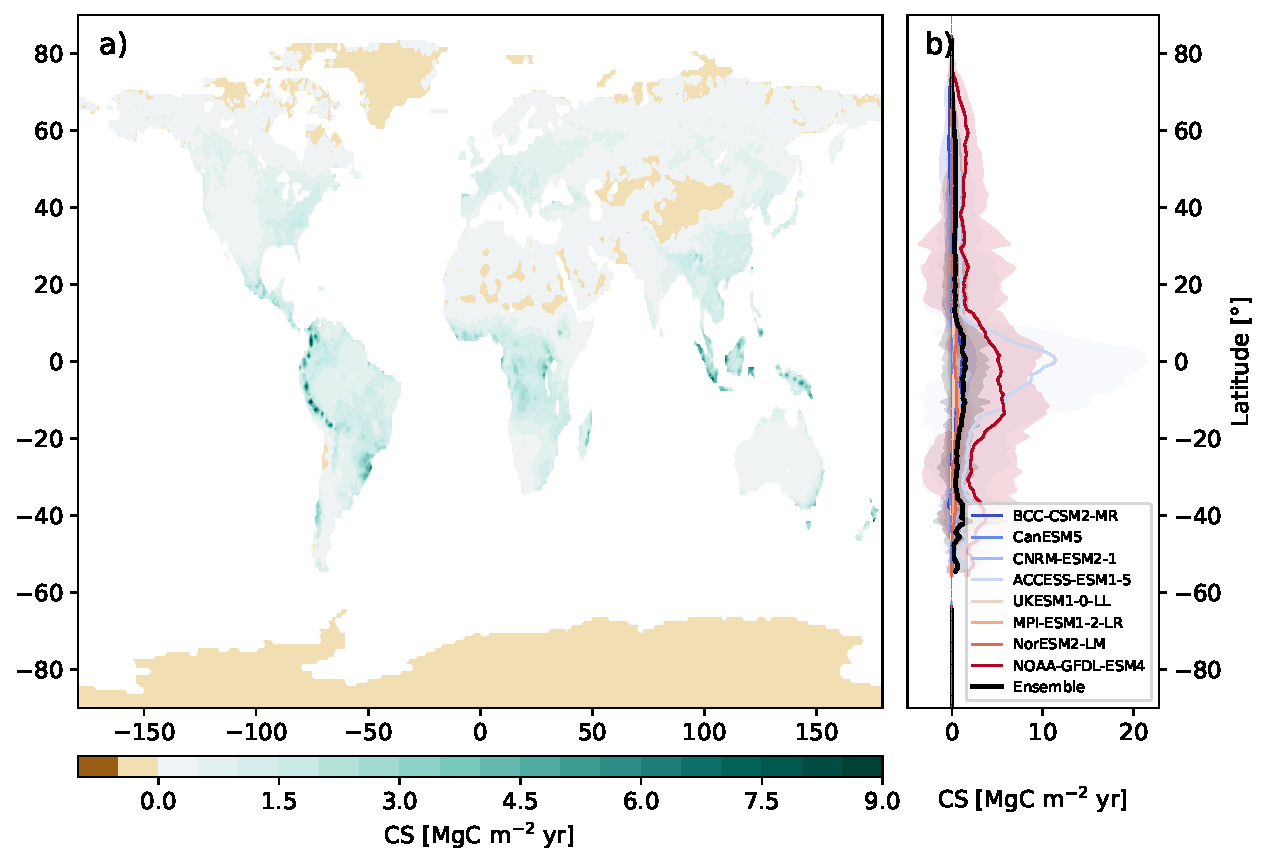
\includegraphics[width=11.4cm]{CMIP6_NEP_CS_map_latitude_mean.pdf}
    \caption{Carbon Sequestration (CS) spatial patterns from NEP from CMIP6 models (1850-2014). a) Global distributions of CS based on the weighted ensemble of 8 CMIP6 models, and b) latitudinal CS profiles for individual CMIP6 models (colored lines) and their ensemble (black line). The dotted line represents zero carbon sequestration and the shadow areas represent two standard deviations from the mean.}
    \label{fig:CMIP6_NEP_map}
\end{SCfigure*}

The cumulative CS across latitudinal zones exhibits a consistent trend over time in all models, albeit with varying magnitudes. NOAA-GFDL-ESM4 and ACCESS-ESM1-5 models show the highest sequestration values, while CanESM5 and BCC-CSM2-MR models show the lowest (Fig.~\ref{fig:CMIP6_NEP_time}a). Tropical regions have sequestered the largest amount of carbon from 1850 to 2014, followed by mid-latitudes (Fig.~\ref{fig:CMIP6_NEP_time}b-d). Although high latitudes sequester on average more carbon per unit area than mid-latitudes (Fig.~\ref{fig:CMIP6_NEP_map}b), the larger territorial expanse of mid-latitudes results in a greater total CS (Fig.~\ref{fig:CMIP6_NEP_time}). All CMIP6 models indicate a positive CS in the tropics during the studied period (Fig.~\ref{fig:CMIP6_NEP_time}b). However, in mid- and high-latitudes, at least one model (BCC-CSM2-MR) shows negative CS, where accumulated respiration exceeds GPP (Fig.~\ref{fig:CMIP6_NEP_time}c,d). Additionally, three models indicate nearly zero CS in high latitudes (Fig.~\ref{fig:CMIP6_NEP_time}d).

\begin{figure}%[\sidecaptionrelwidth][t!]
    \centering
    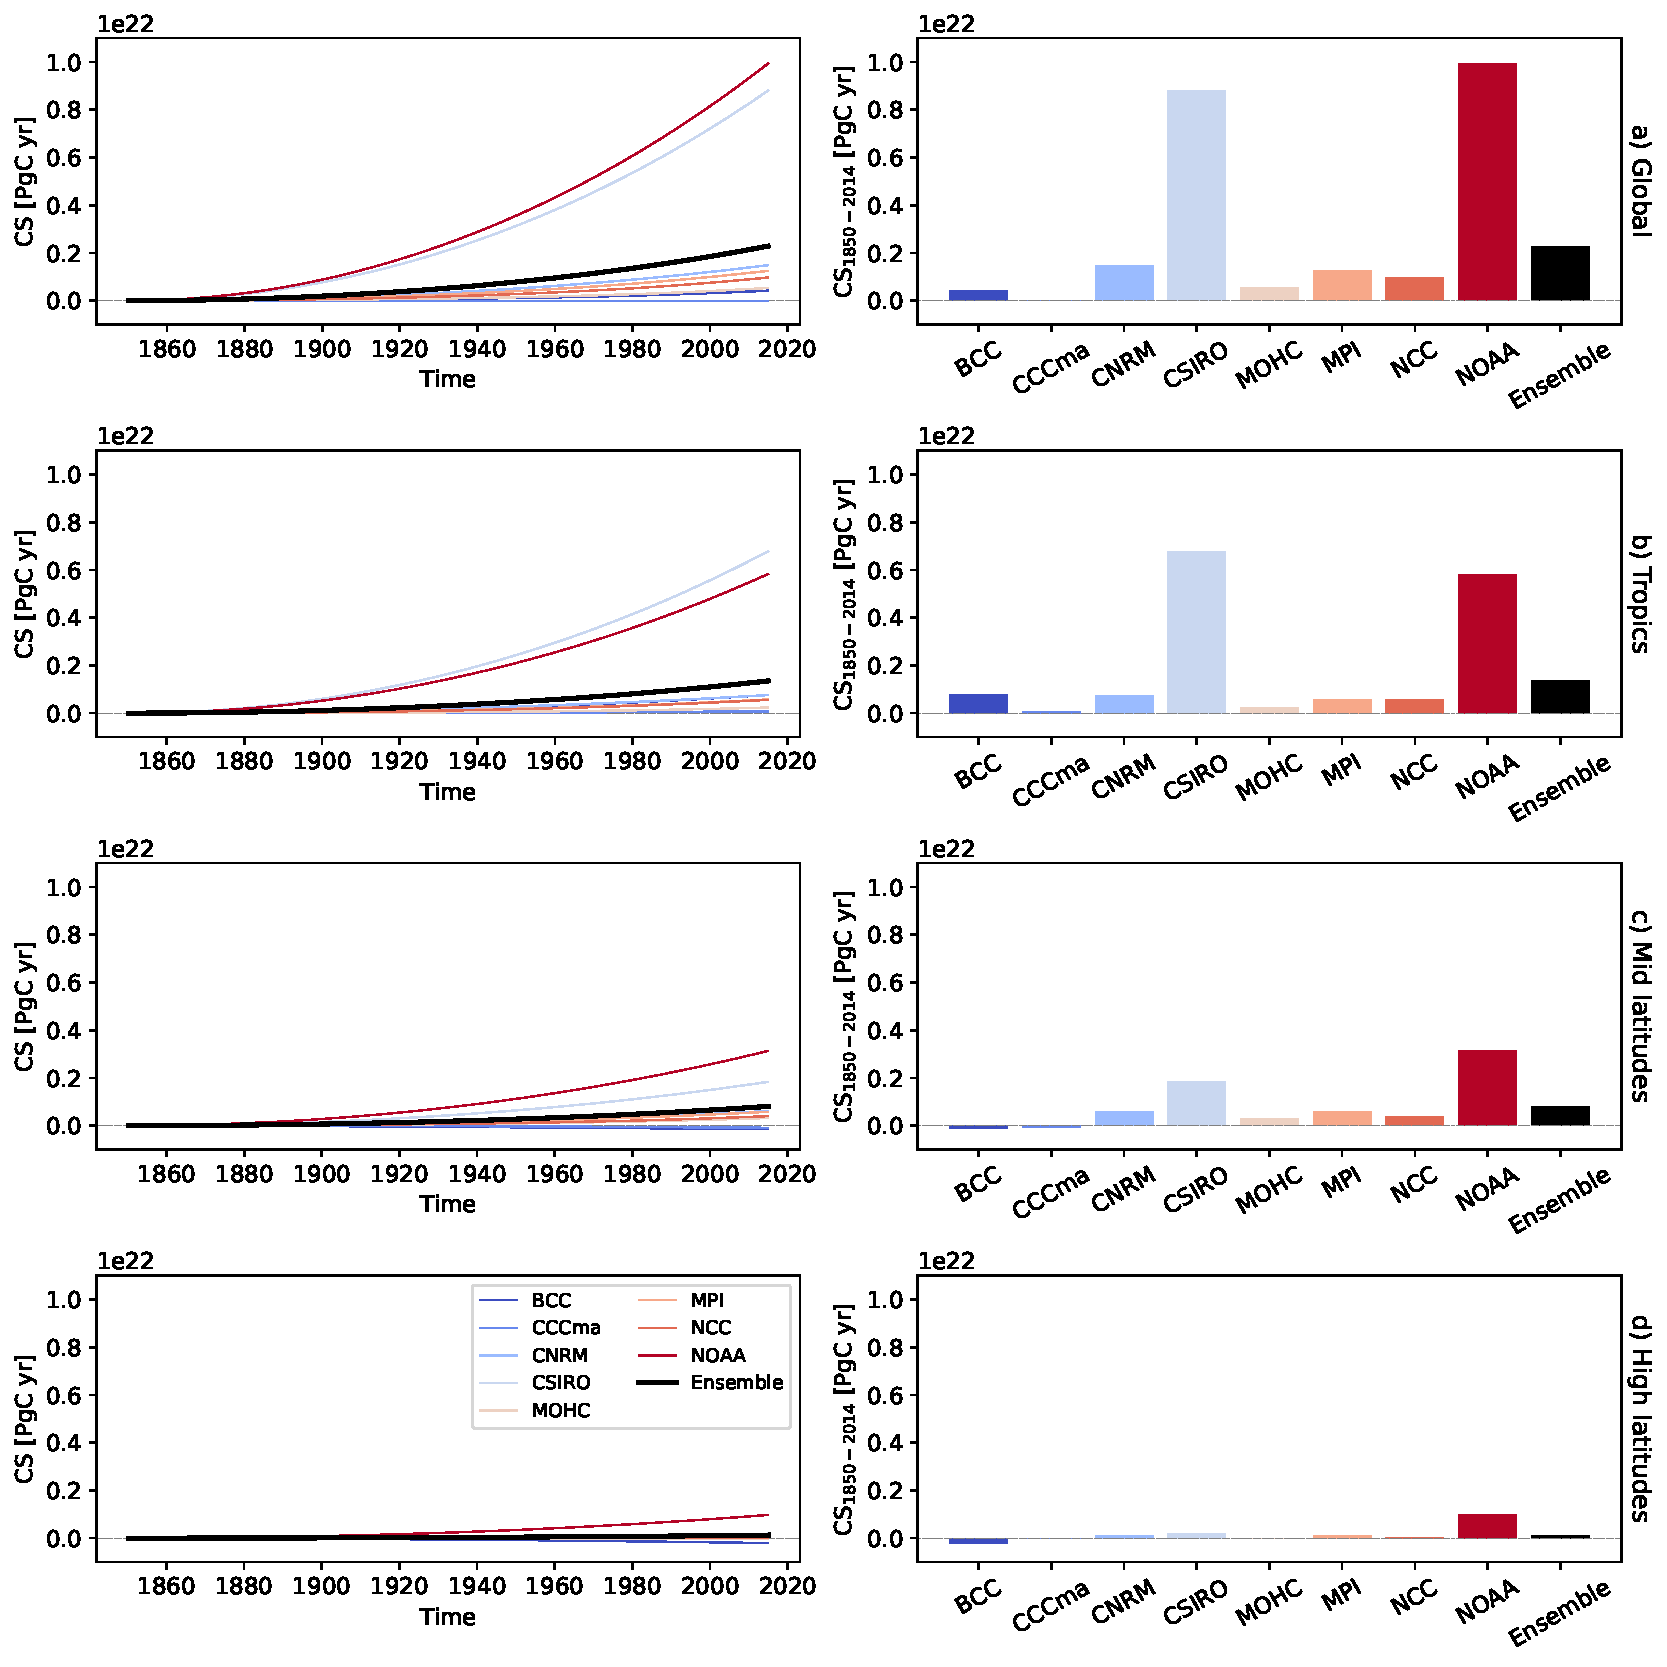
\includegraphics[width=1.0\linewidth]{CMIP6_NEP_CS_time_final.pdf}
    \caption{Time accumulation of Carbon Sequestration (CS) (left panel) and CS at the end of the period from 1850 to 2014 (right panel) calculated using NEP for a) global, b) tropics, c) mid-latitudes, and d) high-latitudes zones calculated using the results of 8 models from CMIP6. Black lines and bars indicate the results using the ensemble of the models. The dotted lines indicate null values of CS. To save space, only the initial part of each model name is displayed on the horizontal axes in the right panel. }
    \label{fig:CMIP6_NEP_time}
\end{figure}

\subsection*{Disturbance impacts on Carbon Sequestration} 
The previous results, based on NEP, only account for climate variations and exclude disturbances like deforestation and fires. When using Net Biome Production (NBP) to calculate CS instead, CS dynamics change significantly. The values of CS calculated with NBP are about two orders of magnitude smaller than with NEP (Figs.~\ref{fig:CMIP6_NEP_time}a and ~\ref{fig:CMIP6_NBP_time}a) and are predominantly negative. Globally accumulated CS is negative for all CMIP6 models except CNRM-ESM2-1 and ACCESS-ESM1-5, with the ensemble indicating a carbon debt of approximately 0.8 PgC yr from 1850-2014 (Fig.~\ref{fig:CMIP6_NBP_time}a). This indicates that terrestrial ecosystems lost more carbon than they gained during this period. High latitudes show the least negative values, followed by the tropics (Fig.~\ref{fig:CMIP6_NBP_time}b-d). Negative CS values are observed in 5 out of 8 models for the tropics, 6 for mid-latitudes, and 5 for high latitudes (Fig.~\ref{fig:CMIP6_NBP_time}b-d). Notably, the ensemble accumulation of CS over time is no longer monotonic as when using NEP; after decreasing from 1850 to around 1970, it slightly increases. 

\begin{figure}
    \centering
    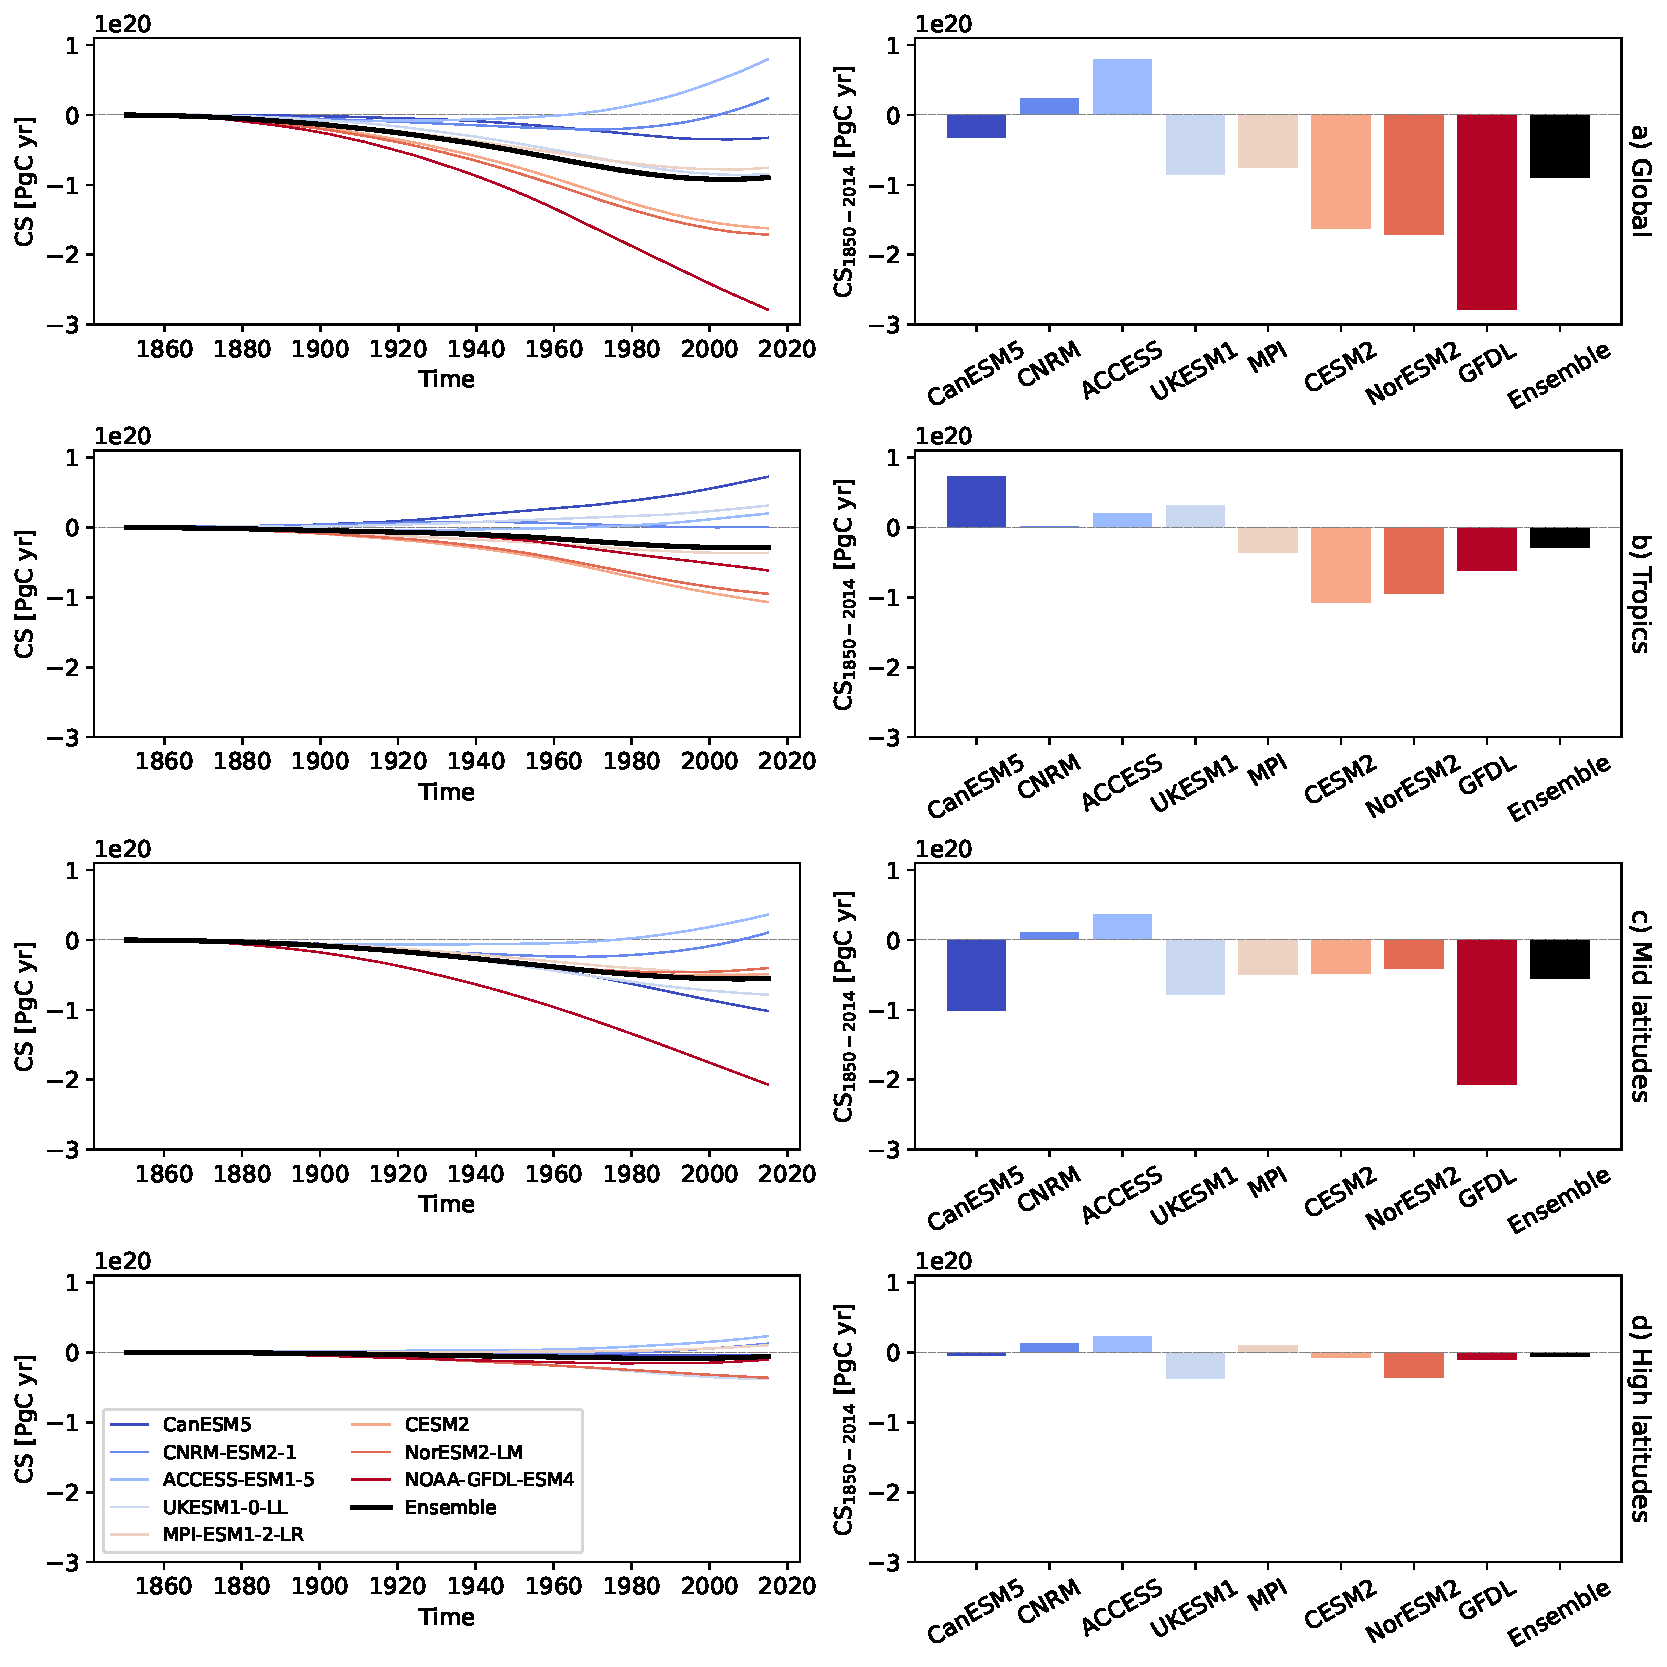
\includegraphics[width=1.0\linewidth]{CMIP6_NBP_CS_time_final.pdf}
    \caption{Time accumulation of Carbon Sequestration (CS) (left panel) and CS at the end of the period from 1850 to 2014 (right panel) calculated using NBP for a) global, b) tropics, c) mid-latitudes, and d) high-latitudes zones calculated using the results of 8 models from CMIP6. Black lines and bars indicate the results using the ensemble of the models. The dotted lines indicate null values of CS. To save space, only the initial part of each model name is displayed on the horizontal axes in the right panel.}
    \label{fig:CMIP6_NBP_time}
\end{figure}

\subsection*{Comparison of CMIP6 carbon sequestration with other data- and model-based products}

Carbon Sequestration calculations for 2001-2014 consistently show higher values when derived from NEP compared to NBP (left and right panel of Fig.~\ref{fig:Comparison_models}, respectively). NEP-based CS from CMIP6, TRENDY, and FLUXCOM-X indicate that tropical regions have the highest values, while high latitudes have the lowest, aligning with previous results in Fig.~\ref{fig:CMIP6_NEP_time}. CMIP6 ensemble yields the highest global CS values, while TRENDY shows the lowest. Although both ensemble models display similar latitudinal zone trends, CMIP6 consistently surpasses TRENDY by up to 250 PgC globally. This substantial difference observed despite some TRENDY models being used in CMIP6 Earth System Models underscores the impact of coupling terrestrial models with climate models and the explicit modeling of carbon movement throughout the Earth System in CMIP6. Then, when using NBP, mid-latitudes show the highest CS values for CMIP6, TRENDY, and CAMS, but not for CarboScope (left panel in Fig.~\ref{fig:Comparison_models}). This finding is consistent with the CMIP6 results for the 1850-2014 period. However, when examining the common 14-year timeframe (2001-2014) across all products, CS values are predominantly positive, except for CAMS in tropical regions. This shift towards positive values likely stems from the increasing trend in CS observed in Fig.~\ref{fig:CMIP6_NBP_time} from around 1970 onwards.  In this shorter timeframe, tropical regions shift from having the second-highest CS to the lowest, with CAMS even indicating a negative value. For NBP-based calculations, data-driven models (CAMS and CarboScope) show higher CS values than the model-based products. CMIP6 and TRENDY yield similar CS values when using NBP, with CMIP6 slightly higher, but the difference is less pronounced compared to NEP-based calculations.

\begin{figure}
    \centering
    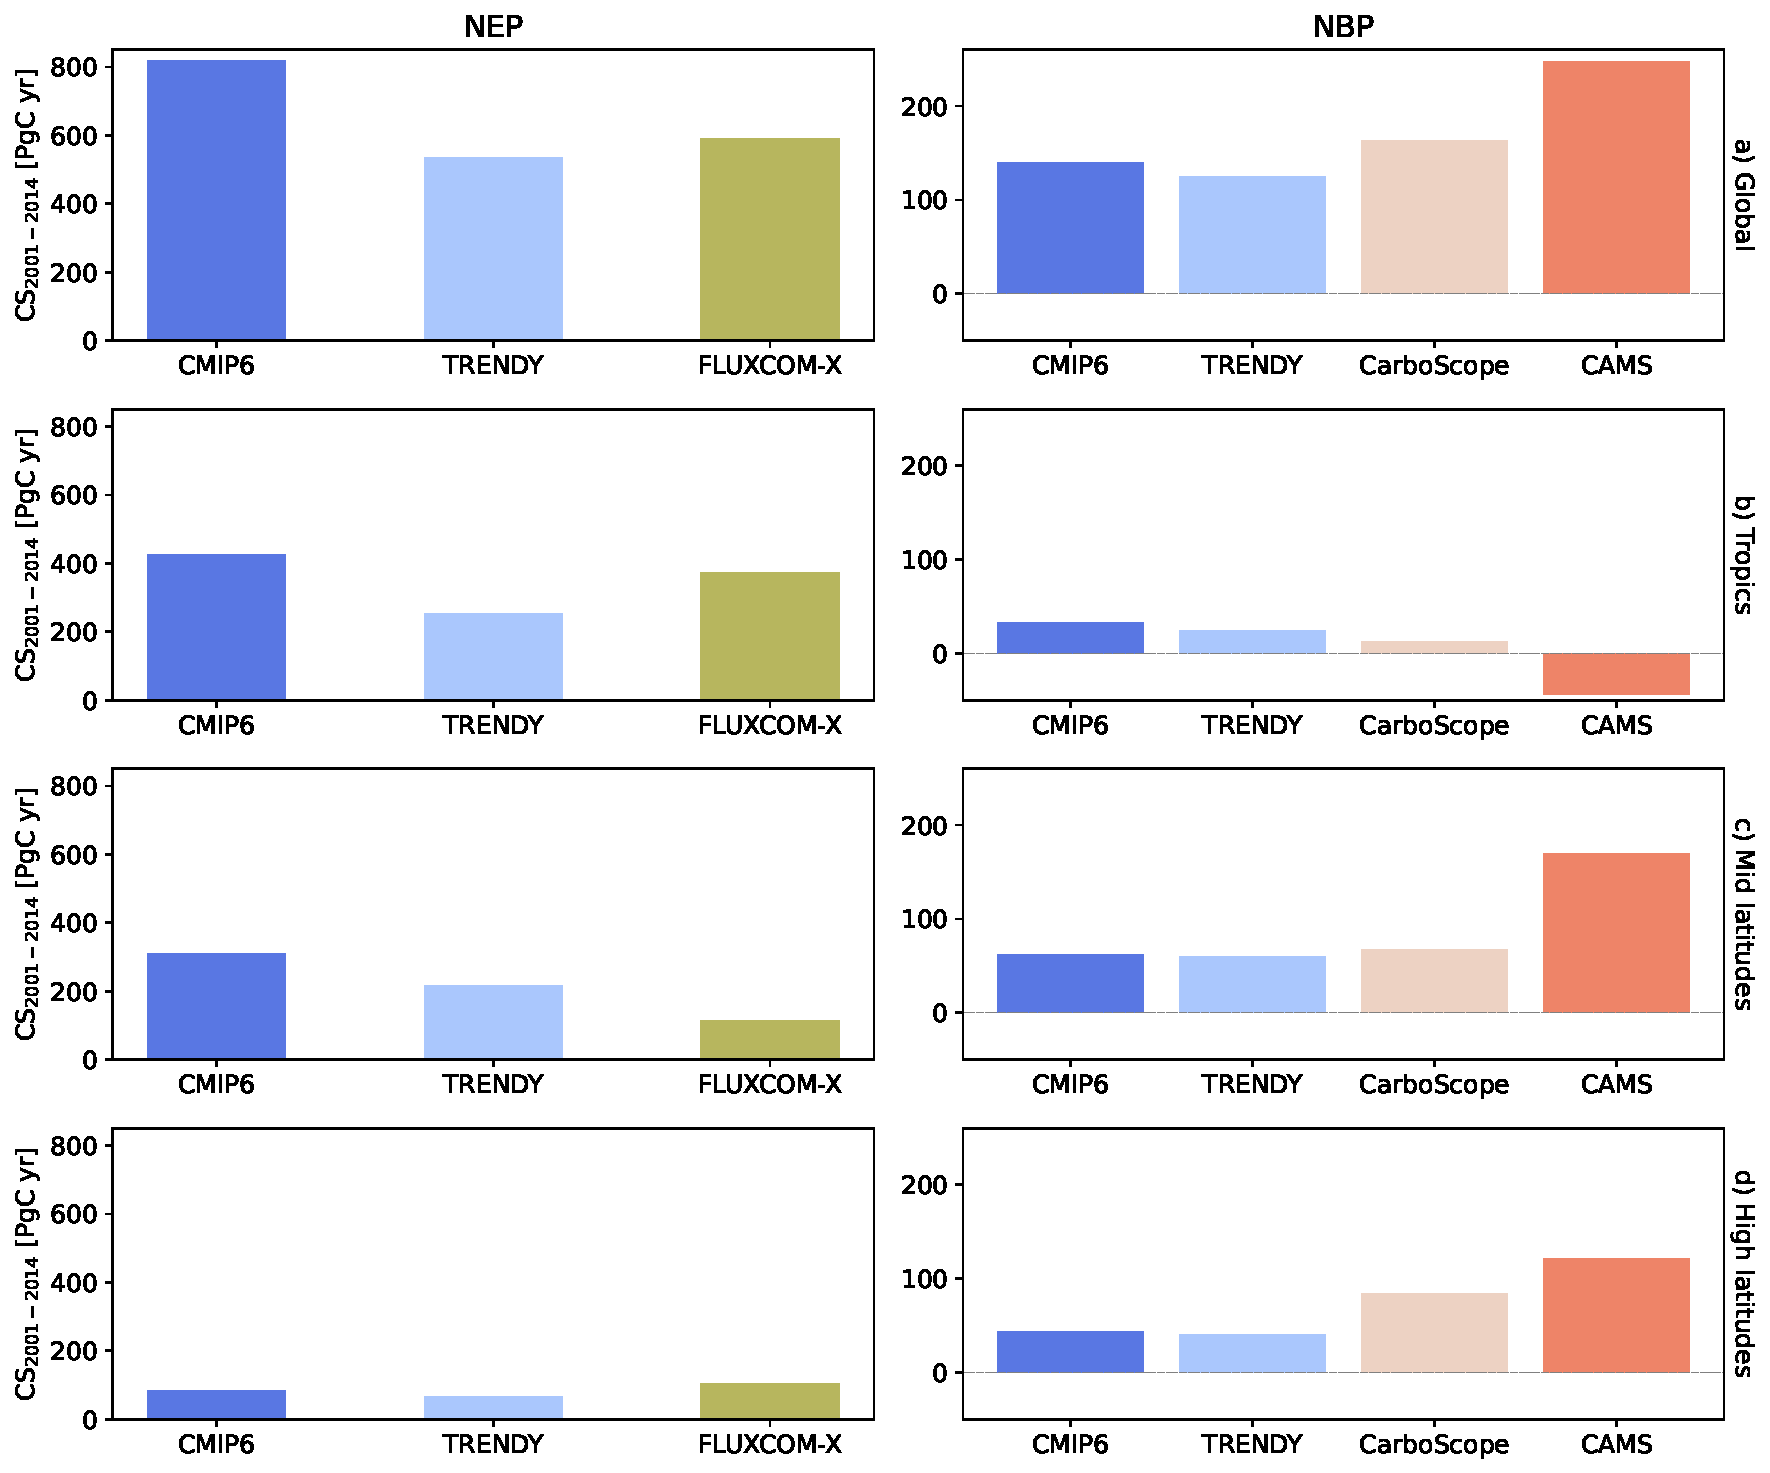
\includegraphics[width=1.0\linewidth]{Comparison_NEPvsNBP.pdf}
    \caption{Carbon sequestration (CS) across different products (2001-2014) calculated using NEP or NEE (left panel) and NBP (right panel) for a) global, b) tropics, c) mid-latitudes, and d) high-latitudes. The dotted lines indicate the null values of CS. CMIP6 and TRENDY CS values correspond to the ensemble of their respective models. Note that the y-axis of the left and right panels do not have the same scale.}
    \label{fig:Comparison_models}
\end{figure}

\section*{Discussion}

\subsection*{Trade-off high carbon assimilation and low respiration}
Terrestrial ecosystems worldwide have absorbed more carbon than released from 1850 to 2014, acting as net carbon sinks when disturbances are not considered. This is evident from the positive CS values across all latitudes (Fig.~\ref{fig:CMIP6_NEP_map}b) and the steady increase in the left panel in Fig.~\ref{fig:CMIP6_NEP_time}. These findings align with the growing global carbon budget and previous research that has observed increases in NEP over various periods and using different methods and databases \cite{Fernandez-Martinez2019,Walker2021,Zhu2022,Ruehr2023}. Several factors explain this trend, including increased atmospheric CO$_2$, higher nitrogen deposition, and the effects of climate change. These factors enhance photosynthesis via fertilization, improve plant water use through reductions in stomatal conductance in water-limited ecosystems, reduce cold limitations at high latitudes, and extend growing seasons \cite{Fernandez-Martinez2017,Fernandez-Martinez2019,OSullivan2019,Friedlingstein2023,Ruehr2023}. While elevated CO$_2$ can positively and negatively affect carbon sequestration, the overall impact up to 2014 appears positive (right panel in Fig.~\ref{fig:CMIP6_NEP_time}). The trends remain consistent even when focusing solely on the 2001-2014 period (Left panel in Fig.~\ref{fig:Comparison_models}).


The high CS observed in forests during the studied period (Fig.~\ref{fig:CMIP6_NEP_map}a) supports earlier research indicating that forests, particularly tropical and boreal regions, are the primary reservoirs of the world's biomass carbon \cite{Xu2021}. This is likely because forests are dominated by trees with large woody masses, and most of the carbon captured by vegetation is allocated to woody tissues \cite{Lu2025}. Their complex structure also makes forests highly efficient at capturing carbon, and when vegetation dies, it contributes to soil organic carbon, further enhancing storage \cite{Sha2022}. Over time, increases in NEP have been observed in forests, especially in those without nutrient limitations \citep{Sitch2015,Fernandez-Martinez2017, Fernandez-Martinez2019}.

The tropics show higher carbon sequestration values when data are divided by latitudinal zones (Figs.~\ref{fig:CMIP6_NEP_map}b and \ref{fig:CMIP6_NEP_time}b), indicating that high tropical assimilation outweighs low respiration in extratropical regions when only climate is considered. This can be attributed to the dense vegetation, extensive biomass, and rapid growth in tropical areas, which contribute significantly to NEP trends \cite{Fernandez-Martinez2019,Xu2021,Ruehr2023,Nelson2024,Sitch2024}, even with rising temperatures and lower simulated soil carbon stocks and residence times \cite{Ito2019,Zhang2025}. High and stable temperatures in these regions promote increased carbon allocation in the canopy \cite{Lu2025}. However, it's important to note that CMIP6 models don't capture potential declines in tropical forest carbon sink strength due to saturation and drought, as suggested by some studies \cite{Koch2021,Friedlingstein2023,Sitch2024}. In contrast, high latitudes ($>$50$^\circ$) exhibit lower CS values, likely due to temperature limitations, although they show enhanced seasonal CO2 cycles with larger summer uptakes and winter releases \cite{Commane2017}. Despite being well-studied, carbon sinks in high-latitude regions still show discrepancies among different products, and soil carbon is often underestimated, suggesting a potentially greater carbon sequestration capacity than currently simulated \cite{Varney2022,Friedlingstein2023}.



%Increasing CO2 was the main factor that accounted for the increasing trends in NEP, with a consistent positive temporal contribution for almost all the latitudinal bands considered and for all three data sets  \cite{Fernandez-Martinez2019}.
%Also, increasing temperatures reduced NEP in warm regions but increased NEP in cold regions (Fig. 2). . However, \cite{Fernandez-Martinez2019}

\subsection*{Consequences of disturbances}

When factors beyond climate, such as harvesting, deforestation, and fire, are considered, CS dynamics shift significantly. From 1850 to 2014, most models indicate that cumulative respiration exceeded assimilation \ref{fig:CMIP6_NBP_time}, making terrestrial ecosystems a carbon source rather than a sink. While the Amazon, Congo, and Papua New Guinea forests still exhibit the highest CS values (\textcolor{red}{Supplementary~Fig.~5}), high-latitude regions show the smallest carbon losses (Fig.~\ref{fig:CMIP6_NBP_time}). These dynamics are driven by deforestation, degradation, and drought, especially in the Amazon, as well as the negative effects of climate variability and change \cite{Koch2021,Tagesson2021,Xu2021,Friedlingstein2023,Sitch2024}. Although African tropical forests generally show net carbon gain and intact tropical Americas continue to gain carbon \cite{Xu2021,Friedlingstein2023,Sitch2024} (though the sink is declining \cite{Hubau2020}), northern boreal forests seem to be benefit from climate change and accumulating carbon at higher rates than in the past \cite{Arora2020,Xu2021,Ruehr2023,Sitch2024}.

When only data from 2001-2014 is considered, CS calculated with NBP becomes positive, albeit lower than CS calculated with NEP (Fig.~\ref{fig:Comparison_models}). This trend change could be attributed to increased CO$_2$ fertilization, longer growing seasons, enhanced nutrient cycling and nitrogen deposition, and reforestation efforts \cite{Piao2007,Friedlingstein2023}. The forest transition in the 19th and 20th centuries, followed by forest regrowth in Europe \cite{Friedlingstein2023}, along with land abandonment, preservation, reforestation, and improved land management practices during the second half of the 20th century \cite{Nabuurs2003}, and the acceleration in the increase rate in global temperature in the 1970s \cite{Sitch2024}, likely explain the increased trend in CS observed since around the 1970s (Left panel in Fig.~\ref{fig:CMIP6_NBP_time}). 

Accounting for disturbances, the tropics sequestered the least amount of carbon among latitude zones during 2001-2014 (Right panel in Fig.~\ref{fig:Comparison_models}), with CAMS even indicating a net carbon release. This aligns with previous findings indicating high cumulative land-use emissions in the tropics and that warm climates decrease NBP due to temperature and soil moisture sensitivities \cite{Padron2022,Fernandez-Martinez2023,Friedlingstein2023}. It's also important to acknowledge that while CMIP6 models capture carbon gains from tree growth, they don't accurately represent carbon losses from tree mortality \cite{Koch2021}.

% Warmer temperatures increase photosynthesis over mid- to high-latitude regions where photosynthesis is cur- rently limited by temperature and more so with increasing CO2 but decrease photosynthesis over tropical regions where the temperatures are already too warm for optimal photosyn- thesis. \cite{Arora2020}

%In contrast to growing fossil emissions, CO2 emissions from land use, land-use change, and forestry remained relatively constant over the 1960–1999 period \cite{Friedlingstein2023}
%DGVM-based estimates include the loss of additional sink capacity, which grows with time.  \cite{Friedlingstein2023}



\subsection*{Agreement and discrepancies among products}

Carbon Sequestration (CS) values vary significantly among CMIP6 models and different products, as previously noted by researchers using various carbon metrics \cite{Arora2020,Melnikova2021,Varney2022,Zhu2022}. The behavior of CMIP6 models is influenced by their response to CO$_2$, temperature perturbations, resolutions, residence times, land surface schemes, and the inclusion of components such as nutrient cycles, fires, and dynamic vegetation \cite{Ito2019,Arora2020,Hu2022,Zechlau2022}. Models that couple the nitrogen (N) cycle are expected to reduce CO$_2$ fertilization and carbon releases, show a lower negative impact of global warming, and align better with observations \cite{Zechlau2022,Gier2024}. In a different CMIP6 experiment (1pctCO2), Arora et al. \cite{Arora2020} found that CNRM-ESM2-1 and CanESM5 have the largest land carbon uptake, which only slightly aligns with our CS-NBP results (Fig.~\ref{fig:CMIP6_NBP_time}). Melnikova et al. \cite{Melnikova2021} also identified CNRM-ESM2-1 as the model with the highest land carbon uptake. These models are not coupled with the N cycle, leading to fewer limitations on photosynthesis. CanESM5 exhibits a strong CO$_2$ fertilization effect due to retuned photosynthesis parameters and high carbon use efficiency \cite{Arora2016}, while CNRM-ESM2-1 shows high land carbon uptake attributed to its long carbon residence time in soils and vegetation \cite{Arora2020}. Arora et al. \cite{Arora2020} also found ACCESS to have the lowest land carbon uptake, citing weak CO$_2$ fertilization due to nutrient limitations from N and P coupling. However, our study shows ACCESS as one of the models with the highest CS values, being one of the few models indicating positive CS-NBP, and CNRM-ESM2 and CanESM5 do not demonstrate notably high CS values  (Figs.~\ref{fig:CMIP6_NEP_time} and \ref{fig:CMIP6_NBP_time}). These differences likely arise from the definition of CS used in this study. Unlike approaches that focus solely on carbon stocks, this metric considers the long-term carbon input-output balance \cite{Sierra2021}, accumulating effects over time. For example, CS accumulates both the effects of low carbon uptake rates caused by N limitations and the small carbon releases due to additional N release from dead organic matter triggered by global temperature increases \cite{Arora2013,Zechlau2022}, which could explain the high CS values observed in the ACCESS model.

Our analysis did not reveal a clear pattern between models considering N cycle coupling (ACCESS-ESM1-5, CESM2, MPI-ESM1-2-LR, NorESM2-LM, UKESM1-0-L)  and dynamic vegetation (NOAA-GFDL-ESM4, CESM2, and UKESM1-0-LL) and CS values. However, we observed a clear pattern of lower CS-NBP values in models incorporating fire components (NOAA-GFDL-ESM4, NorESM2-LM, CESM2, MPI-ESM1-2-LR) (Fig.~\ref{fig:CMIP6_NBP_time}), except for CNRM-ESM2-1. Notably, the GFDL model shifts from having the highest CS value for NEP to the lowest for NBP (Figs.~\ref{fig:CMIP6_NEP_time} and \ref{fig:CMIP6_NBP_time}). This suggests that the immediate carbon losses from fires outweigh the potential long-term benefits of low-intensity fires in promoting forest carbon storage \cite{Hurteau2019}, or that these long-term effects are not considered in the models. Furthermore, the differences observed between CESM2 and NorESM2-LM results, despite both using the same land model (CLM5), emphasize the complex interactions within the entire Earth system simulation and the intricate nature of Earth system modeling, where even slight differences in parameterizations or representations of processes can lead to divergent results \cite{Argles2022}. The complexity of ESMs, which aim to simulate all relevant physical, chemical, and biological processes, means that uncertainties persist, likely due to models still missing key processes or inadequately representing certain interactions within the Earth system \cite{Varney2022,Shi2024}.

Comparing results from different products for 2001-2014, CMIP6, TRENDY, and FLUXCOM-X agree that CS with no disturbances is highest in the tropics, followed by mid-latitudes (left panel in Fig.~\ref{fig:Comparison_models}). This pattern aligns with findings from the full CMIP6 time series (Fig.~\ref{fig:CMIP6_NEP_time}). CMIP6 ensemble shows the highest global CS values when calculated with NEP, while the TRENDY ensemble shows the lowest as previously noted for carbon land sink \cite{Melnikova2021}. For CS calculated with NBP, CMIP6 remains higher than TRENDY, but the gap narrows (Fig.~\ref{fig:Comparison_models}). The main difference between CMIP6 and TRENDY lies in their nature: CMIP6 is an intercomparison of Earth System Models (ESMs), while TRENDY compares Dynamic Global Vegetation Models (DGVMs). ESMs assimilate physical atmospheric and oceanic data, reproducing historical CO2 growth rates and carbon fluxes between atmosphere, sea, and land \cite{Friedlingstein2023,Li2023}. However, these products are not entirely independent, as some CMIP6 models use TRENDY as land models.

When comparing TRENDY and CMIP6 with data-driven products, it's crucial to recognize that all these approaches have inherent uncertainties stemming from various sources such as modeling assumptions and design choices, forcing datasets, representation of processes, under-sampling in biomes such as tropics, etc. \cite{Ruehr2023}. The FLUXCOM initiative aims to address some of these issues by creating ensemble products and performing cross-consistency checks with independent approaches \cite{Nelson2024}. Our results indicate that inversion products (CAMS and CarboScope) show higher global CS-NBP values than model-based products, except in the tropics. Notably, CAMS even yields negative CS values for the tropics (right panel in Fig.~\ref{fig:Comparison_models}). Explanations for differences between model-based and inversion products include: inadequate parameterization of land management and degradation \cite{Fernandez-Martinez2019}, shorter modeled carbon ecosystem residence time \cite{Wei2022}, insufficient capture of volcanic eruptions effects \cite{OSullivan2021}, underestimation of northern latitude soil carbon stocks \cite{Varney2022}, poor reproduction of forests stocks \cite{Hu2022} and lack of climatic and CO$_2$ interactions \cite{Fernandez-Martinez2019} by model-based products. Despite using weights based on the models' proximity to FLUXCOM-X (for NEP) and CarboScope (for NBP) when calculating the CMIP6 and TRENDY ensembles, the results from these two model groups still show substantial differences.

In the tropics, higher CS-NBP values in CMIP6 and TRENDY compared to inversion products (Fig.~\ref{fig:Comparison_models}b) might be due to models not correctly balancing CO2 fertilization effects and respiration costs in Amazon, inaccurate representation of mortality trends in tropical forests \cite{Koch2021}, overestimation of biomass in tropical forests \cite{Yang2023}, a general tendency to overestimate carbon in tropical regions while underestimating it in the Northern Hemisphere \cite{Gier2024}, and an underestimation of drought impacts on tropical forest ecosystems \cite{Sitch2024}.

Differences between CAMS and CarboScope inversions may stem from varying interhemispheric transport models or inversion settings \cite{Fernandez-Martinez2019}, though the exact reasons remain unclear \cite{Fernandez-Martinez2023}. While this study didn't directly compare FLUXCOM-X with inversion models, previous research found agreements between FLUXCOM-X and CarboScope for 2015-2020 \cite{Nelson2024}. FLUXCOM-X shows higher CS values for high latitudes compared to TRENDY and CMIP6, possibly due to its incorporation of more observational data, which may better capture complex processes in northern extra-tropics \cite{Friedlingstein2023}.












%Comparison with OCO-2 and CarboScope inversions also indicates a substantial improvement of the global mean sea- sonal cycle of NEE (Fig. 5)


%The assess- ment of the net land–atmosphere exchange from DGVMs and atmospheric inversions also shows substantial discrep- ancy, particularly for the estimate of the net land flux over the northern extra-tropics. This discrepancy highlights the dif- ficulty of quantifying complex processes (CO2 fertilization, nitrogen deposition and fertilizers, climate change and vari- ability, land management, etc.) that collectively determine the net land CO2 flux. Resolving the differences in the North- ern Hemisphere land sink will require the consideration and inclusion of larger volumes of observations. Eddy covariance data consisted of 294 sites from around the world though skewed towards a higher representation of tem- perate forests from North America and Europe.For the generation of global flux maps we used hourly meteo- rological data from ERA5 global reanalysis products at 0.25° . measurements of the MODerate Imaging Spectroradiometer (MODIS) of surface reflectance and land surface temperature from collection 006 at daily resolution. Machine learning All X-BASE products are based on gradient-boosted regres- sion trees using the XGBoost library (Chen and Guestrin, 2016). X\cite{Nelson2024}



%The X-BASE product estimates the global terrestrial NEE to be −5.75+-0.33 PgC yr-1 (2001–2020), with hotspots of strong CO2 flux into the ecosystems in the tropical re- gions and temperate regions of North America and Eu- rope (Fig. 4). In contrast to both RS and RS+METEO, India and some regions in central Sahel show prominent patterns of a mean CO2 flux from the ecosystems to the atmosphere in X-BASE, corresponding mostly to crop- designated areas (Fig. C2). 

%However, X-BASE global ter- restrial NEE (−5.63 PgC yr-1) agrees well with the inver- sion estimates of OCO-2 (−4.12 PgC yr-1) and CarboScope (−3.46 PgC yr-1) over the common period (2015–2020). Here, GFED 4.1 (Randerson et al., 2017) emission estimates have been used to correct the inversion estimates for fire emissions. Comparison with OCO-2 and CarboScope inversions also indicates a substantial improvement of the global mean sea- sonal cycle of NEE (Fig. 5) in X-BASE compared to RS and RS+METEO. The systematic bias present in RS and RS+METEO has essentially disappeared in X-BASE. The shape, and in particular the amplitude, of the global NEE seasonal cycle of X-BASE is more consistent with the in- versions. The larger and more realistic seasonal cycle am- plitude of global NEE in X-BASE originates primarily from improved and increased amplitudes in boreal regions.




 











%No dynamic vegetation>  i.e. concurrent, bidirectional transformations between land-use types within a grid cell are not considered; Ito et al., 2020), which may lead to an underestimation of the magnitude of land-use change emission as pointed out previously (e.g., Ciais et al., 2022; Friedlingstein et al., 2021)

%% CMIP6 models.

% --CMIP6-NEP
% Higher CS: GFDL and ACCESS. It is maintained for Tropics and mid latitudes. At high latitudes, GFDL continues to have the largest values.
% GFDL: No N cycle. Dynamic vegetation and fires.
% ACCESS: Cycles of N and P. No fires no dynamic vegetation.

% Lower CS: BCC, CanESM, UKES. It is maintained for TRopics and mid latitudes. Besides for mid latidues and high latidues, BCC and CanESM have negative values.
% BCC: No N, no Dynamic vegetation and no fires.
% CanESM: No N, no Dynamic vegetation and no fires.
% UKES: cycle of N, dynamic vegetation, no fires.

% - CMIP6-NBP
% Higher CS: CNRM and ACCESS. CNRM has null CS in tropics and positive values in mid and high latitudes. And ACCESS have positive values in the three latitudinal zones, being the largest in mid latidudes and the lower in tropics. 
% CNRM:implicit N, no dynamic vegetation and yes fire.
% ACCESS: Cycles of N and P. No fires no dynamic vegetation.

% Lower CS: GFDL, NorESM, CESM2. GFDL only continues being particularly low in mid latidues while NorESM and CEM2 in tropics. In high latidues, CESM2 is much less negative than NorESM2.
% GFDL: No N cycle. Dynamic vegetation and fires.
% NorESM: cycle of N, NO dynamic vegetation, fires.
% CESM2: cycle of N, dynamic vegetation, fires. 
% NorESM and CESM2 have the same land model % Note that CESM2 and NorESM2-LM employ the same land surface component – version 5 of the Community Land Model (CLM5) – so we expect the land carbon cycle to respond very similarly in the two mod- els. Arora

% The inclusion of N cycle does not universally imply lower C uptake as in the case of GFDL. \cite{Arora2020}

% Note that  employ the same land surface component – version 5 of the Community Land Model (CLM5) – so we expect the land carbon cycle to respond very similarly in the two mod- els. Arora

%UKES: 
% Lower ACCESS followed by UKESM. A.
%high-climate-sensitivity models A.
%Compared to its predeces- sor HadGEM2-ES, UKESM1-0-LL represents a prognostic treatment of terrestrial nitrogen including its impact on car- bon storage in vegetation biomass and soil organic matter. A limitation on terrestrial productivity from available nitrogen is likely also the main reason for reduced land carbon storage in UKESM1-0-LL compared to in HadGEM2-ES
% The CO2 fertilization effect is strongest for the three models that simulate vegetation cover dynamically (NOAA-GFDL-ESM4, MPI-ESM1.2-LR, and UKESM1-0-LL) since the ?GPP term also implicitly in- c? cludes the effect of increasing vegetation cover as CO2 in creases. How- ever, these models do not simulate the largest land carbon uptake because of their lower-than-average τveg? and τsoil? values.  The ?GPP  term is unable to capture the CO2 fertilization effect separately from increasing vegetation cover, and this illustrates the challenge in comparing models that do and do not simulate vegetation cover dynamically.  A.

%GFDL: 
%Inclusion of the N cycle does not universally im- ply lower land C uptake. IPSL-CM6A-LR and NOAA-GFDL-ESM4, both of which do not include the land N cycle, yield lower land carbon uptake than four of the mod- els that do include the land N cycle.
%The CO2 fertilization effect is strongest for the three models that simulate vegetation cover dynamically (NOAA-GFDL-ESM4, MPI-ESM1.2-LR, and UKESM1-0-LL) since the ?GPP term also implicitly in- c? cludes the effect of increasing vegetation cover as CO2 in creases. The tree cover in the NOAA-GFDL-ESM4 model, for example, increases in the BGC simulation – particularly in dry, high-latitude regions above 50◦ N (not shown).  The ?GPP  term is unable to capture the CO2 fertilization effect separately from increasing vegetation cover, and this illustrates the challenge in comparing models that do and do not simulate vegetation cover dynamically. A.

%ACCESS:
%ACCESS-ESM1-5, addi- tionally includes a phosphorus cycle.
% Lower ACCESS followed by UKESM. A.
%This Over land, photosynthesis is also affected by temperature (with widely varying responses between models) in addition to respiration, and the γL values vary widely between mod- els between the RAD–BGC and RAD–COU approach and the BGC–COU approach. This is seen, for example, for the ACCESS-ESM1.5, IPSL-CM6A-LR, and CanESM5 models. A.
%The ACCESS-ESM1.5 model exhibits the lowest land car- bon uptake because of its weak CO2 fertilization effect and the lowest CUE? of all models. A.

%BCC:
% BCC: larger dependence of global totale turnover timjje of soil carbon on global warming  \cite{Varney2020}
% canESM5 higher land uptake, followed by BCC.
%hree models with the largest land carbon uptake (CNRM-ESM2-1, BCC-CSM2-MR, and CanESM5) which do not include land the N cycle. A

%CanESM:
%models showing very low (CanESM5) GPP responses  \cite{Zechlau2022}
% high-climate-sensitivity models A.
%hree models with the largest land carbon uptake (CNRM-ESM2-1, BCC-CSM2-MR, and CanESM5) which do not include land the N cycle. A
% CanESM5, a model with the largest land carbon uptake among CMIP6 models. The reason for this is an increase in the strength of its CO2 fer- tilization effect following the retuning of its photosynthesis downregulation parameters, using carbon budget constraints over the historical period, as explained in Arora and Scinocca (2016). CESM1, A.
% Over land, photosynthesis is also affected by temperature (with widely varying responses between models) in addition to respiration, and the γL values vary widely between mod- els between the RAD–BGC and RAD–COU approach and the BGC–COU approach. This is seen, for example, for the ACCESS-ESM1.5, IPSL-CM6A-LR, and CanESM5 models. A.

%The CanESM5 model exhibits higher-than-average land carbon uptake despite its near-average strength of the CO2 fertiliza- tion effect and τveg? and τsoil? values. However, its CUE? is the highest, and therefore a much larger fraction of GPP is converted to NPP. A.
% The largest increase in the vegetation carbon pool is seen in the CanESM5 model that more than compensates for the carbon loss from the soil+ litter carbon pool, yielding a positive value of γL in contrast to other mod- els. This case is one of the few times a positive value of γL is seen in an Earth system model. Thornton et al. (2009) re- ported positive γL after their first attempt to include N cycle in the CLM. Preliminary analysis of CanESM5 data shows the increase in vegetation carbon in the COU relative to the BGC simulation is caused by the increase in GPP and the resulting vegetation growth at middle to high latitudes in re- sponse to warming temperatures and increasing CO2. A.


%CNRM:
% CNRM-ESM2-1 estimates the highest cumulative land carbon uptake and the least cumulative ocean carbon uptake for the 1850–2014 period \cite{Melnikova2021}.

% The distinct changes in CNRM-ESM2-1 in the idealized scenarios were discussed by Arora et al. (2020) and attributed to the larger nonlinearity effects compared to other models\cite{Melnikova2021}

%showing very high (CNRM-ESM2-1) GPP responses  C \cite{Zechlau2022}

%high-climate-sensitivity models A.

%hree models with the largest land carbon uptake (CNRM-ESM2-1, BCC-CSM2-MR, and CanESM5) which do not include land the N cycle. A
% CNRM-ESM2-1 model has the highest land carbon uptake among all models in the BGC simulation. However, this is not caused by a strong CO2 fer- tilization effect (the ?GPP % c? term) but rather by the relatively % high τveg? and τsoil? values. A.

% CNRM-ESM2-1 estimates the highest cumulative land carbon uptake and the least cumulative ocean carbon uptake for the 1850–2014 period \cite{Melnikova2021}. showing very high (CNRM-ESM2-1) GPP responses  C \cite{Zechlau2022} high-climate-sensitivity models A.

% CNRM-ESM2-1 model has the highest land carbon uptake among all models in the BGC simulation. However, this is not caused by a strong CO2 fer- tilization effect (the ?GPP  c? term) but rather by the relatively  high tauveg? and tausoil? values. A

%CESM2: 
%high-climate-sensitivity models A.
%CLM5 (land model of CESM and NCC) on the one hand and the reduc- tion in its nutrient constraints on photosynthesis and the para- metric controls on fertilization responses on the other are discussed in Wieder et al. (2019) and Fisher et al. (2019), 

%MPI:
%For the MPI ESM, the decrease in land carbon uptake in MPI-ESM-LR for CMIP5 and MPI-ESM1.2-LR for CMIP6 is associated with the implementation of a nitro- gen cycle model (Goll et al., 2017) and a new soil carbon model Yasso (Goll et al., 2015).  A.
% The CO2 fertilization effect is strongest for the three models that simulate vegetation cover dynamically (NOAA-GFDL-ESM4, MPI-ESM1.2-LR, and UKESM1-0-LL) since the ?GPP term also implicitly in- c? cludes the effect of increasing vegetation cover as CO2 in creases. How- ever, these models do not simulate the largest land carbon uptake because of their lower-than-average τveg? and τsoil? values.  The ?GPP  term is unable to capture the CO2 fertilization effect separately from increasing vegetation cover, and this illustrates the challenge in comparing models that do and do not simulate vegetation cover dynamically.  A.



% \begin{itemize}
%    \item The cumulative CS across latitudinal zones exhibits a consistent trend over time in all models.  NOAA and CSIRO models show higher CS values and CCCma and BCC the lowest. 
%    \item All CMIP6 models indicate a positive CS (NEP) in the tropics during the studied period (Fig. 2b). In mid- and high-latitudes, at least one model (BCC) shows accumulated respiration exceeds GPP. 
%    \item Globally accumulated CS (NBP) is negative for all CMIP6 models except CNRM and CSIRO.
%    \item Negative CS values are observed in 5 out of 8 models for the tropics, 6 for mid-latitudes, and 5 for high latitudes
%     \item NEP-based CS from CMIP6, TRENDY, and FLUXCOM-X indicate that tropical regions have the highest values, while high latitudes have the lowest, aligning with CMIP6 results for the complete time series.
%     \item CMIP6 ensemble yields the highest global CS (NEP) values, while TRENDY shows the lowest. Although both ensemble models display similar latitudinal zone dynamics, CMIP6 consistently surpasses TRENDY by up to 250 PgC globally. CMIP6 and TRENDY yield similar CS values when using NBP, with CMIP6 slightly higher, but the difference is less pronounced compared to NEP-based calculations.
%     \item When using NBP, mid-latitudes show the highest CS values for CMIP6, TRENDY, and CAMS, but not for CarboScope.
%     \item For NBP-based calculations, data-driven models (CAMS and CarboScope) show higher CS values than the model-based products.
% \end{itemize}






\subsection*{Implications for climate change mitigation}
\begin{itemize}
    \item Importance of temporal scale consideration. The research underscores the importance of considering both carbon inputs and outputs, as well as disturbances when developing climate mitigation strategies involving terrestrial ecosystems.
    \item Disturbances have had a significant impact on terrestrial carbon cycles over the past century, particularly in tropical regions.
    \item Tropical ecosystems have the potential to sequester more carbon than they currently do, suggesting opportunities for enhanced mitigation efforts in these areas.
    \item Different carbon cycle models and data products show varying results, highlighting the need for continued refinement and comparison of these tools.
    \item Understanding the spatial distribution of carbon sequestration potential can help prioritize areas for ecosystem-based mitigation approaches.
\end{itemize}

%The MME consistently outperforms all individual models in nearly every respect. \citet{Hu2022}


%ESMs and DGVMs models still fail to capture some of the interactions that occur in nature. The \cite{Fernandez-Martinez2019}
 
%Dynamic global vegetation models (DGVMs) are state-of-the-art terrestrial ecosystem models that incorporate known physiological and biological mechanisms responsible for ecosystem function and carbon cycling. These models are used to project the future of the Earth System and delineate individual drivers of carbon fluxes into and out of the atmosphere. \cite{Ruehr2023}
%This discrepancy highlights the dif- ficulty of quantifying complex processes (CO2 fertilization, nitrogen deposition and fertilizers, climate change and vari- ability, land management, etc.) that collectively determine the net land CO2 flux. Resolving the differences in the North- ern Hemisphere land sink will require the consideration and inclusion of larger volumes of observations. \cite{Friedlingstein2023}

%Many authors agree in uncertainty and intermodel spread in terrestrial C storage is due to resistance time \cite{Arora2020,Wei2022,Varney2022}

%In addition, we find that the detrended interannual variability of projected NBP is better explained by soil moisture than temperature in most models and across most regions. A notable excep- tion is the core of the Amazon, where temperature is more important than soil moisture to explain the interannual vari- ability of NBP in the models. This finding provides explicit evidence that improving the representation of the local-scale sensitivity of NBP to interannual climate variability has the potential to re- duce uncertainty in long-term projections of the global land carbon sink. For example, a high regional contribution of sSM and/or sT to a model’s land sink anomaly indicates the need to evaluate and improve potentially related processes such as water stress on photosynthesis, the effect of temperature and moisture on soil carbon loss due to microbial activity, and the occurrence and magnitude of fire emissions.\citep{Padron2022}

%Despite these regional negative effects of climate change on SLAND, the efficiency of land to remove anthropogenic CO2 emissions has remained broadly constant over the last 6 decades, with a land-borne fraction (SLAND/(EFOS + ELUC)) of around 30% (Fig. 9b). \cite{Friedlingstein2023}

%Comparison of estimates from multiple approaches and observations shows the following: (1) a persistent large uncertainty in the estimate of land-use changes emissions, (2) a low agreement between the different methods on the magnitude of the land CO2 flux in the northern extra-tropics, and (3) a discrepancy between the different methods on the strength of the ocean sink over the last decade. \cite{Friedlingstein2023}

%The loss of carbon from disturbance may not be released to the atmosphere in the year of loss but delayed for years (e.g., timber products) or transferred to other pools (e.g., live to dead) (43). \cite{Xu2021}

%The higher CS values observed in forests (Fig.~\ref{fig:CMIP6_NEP_map}a) underscore the important role of these ecosystems in the global carbon cycle. This means that carbon inputs have been larger than carbon outputs during this time horizon, highlighting the capacity of terrestrial ecosystems to contribute to mitigating anthropogenic carbon emissions. 

%Since 2020 the globe has experienced La Niña conditions,which would be expected to lead to an increased land car- bon sink. A clear peak in the global land sink is not evi- dent in SLAND, and we find that a La Niña-driven increase in the tropical land sink is offset by a reduced high-latitude extra-tropical land sink, which may be linked to the land re- sponse to recent climate extremes. A continuing conundrum is the partitioning of the global atmosphere–land flux between the Northern Hemisphere land and the tropical land (Stephens et al., 2007; Pan et al., 2011; Gaubert et al., 2019). It is of importance because each region has its own history of land-use change, climate drivers, and impact of increasing atmospheric CO2 and nitro- gen deposition. Quantifying the magnitude of each sink is a prerequisite to understanding how each individual driver im- pacts \cite{Friedlingstein2023}

%Global fossil CO2 emissions, EFOS (including the cement carbonation sink), have increased every decade from an av- erage of 3.0+-0.2 GtC yr-1 for the decade of the 1960s to an average of 9.6+-0.5 GtC yr-1 during 2013–2022 (Table 7, Figs. 2 and 5). The growth rate of these emissions decreased between the 1960s and the 1990s, from 4.3%yr-1 in the 1960s (1960–1969), 3.2%yr-1 in the 1970s (1970-1979), 1.6%yr-1 in the 1980s (1980–1989) to 1.0%yr-1 in the 1990s (1990–1999). After this period, the growth rate be- gan increasing again in the 2000s at an average growth rate of 2.8%yr-1, decreasing to 0.5%yr-1 for the last decade (2013–2022). The cumulative land sink is almost equal to the cumulative land-use emissions (220+-70 Gt C), making the global land nearly neutral over the whole 1850– 2022 period\cite{Friedlingstein2023}


%Models show that after the CO2 concentration and air temperature peaks, land and ocean are decreasing carbon sinks from the 2,040s and become sources for a limited time in the 22nd century.The decrease in the carbon uptake precedes the CO2 concentration peak. The early peak of the land uptake occurs due to a larger increase in ecosystem respiration than the increase in gross primary production, as well as due to a concomitant increase in land-use change emissions primarily attributed to the wide implementation of biofuel croplands. \citet{Melnikova2021}

%The difference in mean residence time explains about 88% of the variation of global SOC stock among the models (figure S3). Previous studies have pointed out that the turnover rate is an important metric ofecosystemcar- bon pools (e.g. Bonan et al 2013, Todd-Brown et al 2013, Carvalhais et al 2014, Friend et al 2014).  \citep{Ito2019}

%Although the model results presented here appear inconsistent, nonetheless have implications for soil management for mitigation of global warming. through carbon sequestration. First, the results indic- ate a range of possible rates of global SOC stock change (figure 9; see figure S8 for zonal results). Second, the spatial results showed which regions are likely to respond more sensitively, specific- ally, to land-use change and land management (e.g. figures S5–S7). Third, the simulation results provide supple mentary evidence that prevention of deforestation or reforestation can enhance SOC stocks.  \citep{Ito2019}

% Forest conservation priority: The high carbon sequestration rates in forests, particularly in the tropics, emphasize the urgent need for conservation and sustainable management of these ecosystems.

% Reforestation potential: Areas outside the tropics also show positive sequestration, suggesting that reforestation and afforestation efforts in temperate and boreal regions can contribute meaningfully to carbon mitigation.

% Ecosystem-based approaches: The global nature of carbon sequestration supports the implementation of diverse, ecosystem-based approaches to climate change mitigation across different latitudes.

%Studies estimate that tropical forests alone are responsible for holding back more than 1 degree C of atmospheric warming (The Unseen Effects of Deforestation: Biophysical Effects on Climate, Lawrence et al. 2022)

%n many tropical forest regions, there is a tension between forests and agricultural expansion. In the Amazon rainforest, land grabbing for commodity uses like cattle ranching or soy farming has advanced deforestation. Increasing protected forest areas and strengthening the rights of Indigenous communities to manage their own territories has proven effective at reducing deforestation and its associated emissions in Brazil. “Undesignated lands” have the highest levels of land grabbing and deforestation.

%degradation attributable to selective logging, edge ef- fects or fragmentation is not captured.  \cite{Friedlingstein2023}

% Wildfire—although a natural element in boreal forests—represents one of the greatest threats to boreal forest carbon. With increased temperatures, rising more than twice as fast in boreal forests compared to lower latitudes, and more frequent and long-lasting droughts, boreal forests are now experiencing more frequent and intense wildfires. The hotter and more often a stand of boreal forest catches fire, the deeper into the soil carbon pool the fire will burn, sending centuries-old carbon up in smoke in an instant. Logging of high-carbon primary forests is also a big issue in the boreal.

%Overall, the models suggest that the global and NHL terrestrial ecosystems will be consistent carbon sinks in the future, and the magnitude of the carbon sinks is projected to be larger under scenarios with higher radiative forcing. \citep{Qiu2023}

%Although most CMIP6 models apparently agree on increased soil C storage during the 21st century, this consensus obscures substantial model disagreement on the mechanisms underlying soil C response, calling into question the reliability of model predictions. \citep{Shi2024}

%soil carbon simulations in both the CMIP5 and CMIP6 ESM generations seem to be spuriously highly correlated with NPP, which may make soil carbon in these models over-responsive to future projected changes in NPP. \citep{Varney2022}


%Our results support several previous studies that also identified an underestimation of SOC turnover times in ESMs through 14C observations (He et al., 2016; Shi et al., 2020).]

%to preserve tropical ecosystems should be a global priority to mitigate anthropogenic CO2 emissions. Temperature has diminished the capacity of terrestrial ecosystems to sequester C, which jeopardizes future C sink capacity in light of global warming. So far, our results suggest that the benefit of increasing atmospheric concentrations of CO2 are still compensating the negative ones of temperature rise, in terms of C sequestration. However, if it has not started to change already6 , this pattern may eventually reverse with saturation of land C sinks5,31 or because warm ecosystems tend to decrease NEP as temperature rises (Fig. 2). the comparison between model results indicated that the DGVMs were unable to reproduce several features of the global land C sinks observed in inversion models. Process-based Earth system models will need to improve their parameterization to capture these features to better predict the future of land C sinks. Online \cite{Fernandez-Martinez2019}.

%Changes in NPP are more consistent between models than changes in residence time, which increases, decreases, or does not change over this century. Although it has been recognized for some time that differences in modeled NPP responses to climate and CO2 are major sources of uncertainty in GVMs, there has been little discussion on the importance of residence time. A significant component of this key ecosystem characteristic is dependent on relatively slow processes such as rates of recuitment, mortality, and changes in vegetation composition. In contrast, validation exercises have focused on short-term carbon fluxes and leaf area dynamics, features readily observable (e.g., ref. 18). However, there is in- creasing recognition of the importance of demographic processes not just for compositional dynamics, but also for changes in carbon balance (e.g., ref. 19) Vegetation carbon residence time not only is important because of its contribution to GVM uncertainty, but also represents a key stage in the cascade of carbon from the atmosphere, through various organic and inorganic surface pools, and back to the atmosphere. Changes in vegetation carbon residence times can cause major shifts in the distribution of carbon between pools, overall fluxes, and the time constants of terrestrial carbon tran- sitions, with consequences for the land carbon balance and the associated state of ecosystems. The\cite{Friend2014}

%the emissions from permanent deforestation – the largest of our component fluxes – could be halted (largely) without compromising carbon uptake by forests, contributing substantially to emissions reduction. By con- trast, reducing wood harvesting would have limited poten- tial to reduce emissions as it would be associated with less forest regrowth; removals and emissions cannot be decou- pled here on long timescales. Although the budget imbalance is near zero for the recent decades, this could be due to compensation of errors. W \cite{Friedlingstein2023}


%Since the 1990s, the average growth rate of fossil CO2 emissions has continuously declined across the group of developed countries of the Organisation for Economic Co- operation and Development (OECD), with emissions peak- ing in around 2005 and now declining at around 1%yr-1 (Le Quéré et al., 2021). In the decade 2013–2022, territo- rial fossil CO2 emissions decreased significantly (at the 95% confidence level) in 26 countries/economic entities whose economies grew significantly: Belgium, Brazil, Czechia, Denmark, Estonia, Finland, France, Germany, Greece, Hong Kong SAR, Israel, Italy, Jamaica, Japan, Luxembourg, the Netherlands, Norway, Portugal, Romania, Slovenia, South Africa, Sweden, Switzerland, the United Kingdom, the USA, and Zimbabwe (updated from Le Quéré et al., 2019). Altogether, these 26 countries emitted 2.7 GtC yr-1 (10.0 GtCO2 yr-1) on average over the last decade, about 28% of world CO2 fossil emissions. For comparison, 22 countries showed a significant decrease in territorial fossil CO2 emissions over the previous decade (2003–2012). Fig- ure 16 shows that the emission declines in the USA and the EU27 are primarily driven by slightly weaker economic growth in the last decade compared to the 1990s, sustained declines in energy per GDP (though weakening in the USA), and sustained declines in CO2 emissions per energy unit (de- carbonization) with a slight acceleration in the USA in the last decade. In n contrast, fossil CO2 emissions continue to grow in nonOECD countries, although the growth rate has slowed from more than 6%yr-1 during the 2000s to less than 2%yr-1 in the last decade. Representing 47% of non-OECD emis- sions in 2022, a large part of this slowdown is due to China, which has seen emissions growth decline from 9%yr-1 in the 2000s to 1.6%yr-1 in the last decade. Excluding China, non-OECD emissions grew at 3.1%yr-1 in the 2000s com- pared to 1.5%yr-1 in the last decade. China had weaker economic growth in the 2000s compared to the 2010s and a higher decarbonization rate from 2005 to 2015 that is com- parable to the highs in the 1990s, though the decarboniza- tion rate has slowed considerably since 2016 (Fig. 16). India and the rest of the world have had strong economic growth that is not offset by decarbonization or declines in energy per GDP, driving up fossil CO2 emissions. Despite the high de- ployment of renewables in some countries (e.g. India), fossil energy sources continue to grow to meet growing energy de- mand (Le Quéré et al., 2019) Globally, fossil CO2 emissions growth is slowing, and this is due in part to the emergence of climate policy (Eskander and Fankhauser, 2020; Le Quéré et al., 2019) and technolog- ical change, which are leading to a shift from coal to gas and growth in renewable energies, as well as reduced expansion of coal capacity. At the aggregated global level, decarbonization shows a strong and growing signal in the last decade, with smaller contributions due to lower economic growth and declines in energy per GDP. Altogether, global emissions are still growing (average of 0.5%yr-1 over the 2013–2022 decade) and are far from the reductions needed to meet the ambitious climate goals of the UNFCCC Paris Agreement. \cite{Friedlingstein2023}


%The persistent unexplained variability in the carbon budget imbalance limits our ability to verify reported emissions (Peters et al., 2017) and suggests we do not yet have a com- plete understanding of the underlying carbon cycle dynam- ics on annual to decadal timescales The long-standing sparse data coverage of fCO2 observations in the South- ern Hemisphere compared to the Northern Hemisphere (e.g. Takahashi et al., 2009) continues to exist (Bakker et al., 2016, 2023, Fig. S1) and to lead to substantially higher uncertainty in the SOCEAN estimate for the Southern Hemisphere (Wat- son et al., 2020; Gloege et al., 2021; Hauck et al., 2023).\cite{Friedlingstein2023}

%Estimates that take cost into account suggest that reforestation could increase the land sink by up to 8–13.8 Pg of CO2 equivalents (CO2e) per year (2.3–3.7 PgC yr-1) globally from 2020 to 2050260. This value could even be underestimated if CO2 and climate effects continue to enhance the land sink (for example, ref. 22). However, the value could be overestimated if the impacts of disturbances or cost become large. Reforestation, agroforestry and reducing deforestation together have the potential to mitigate up to 20 PgCO2e yr-1 (Fig. 7a)260 . The main policy tool aimed at reforestation and reduced deforestation is carbon credits22 , which assign monetary value to carbon captured from, or emissions prevented to, the atmosphere. The general consensus is that protecting old-growth forests is optimal for carbon storage because existing forests, even when old, continue to act as net land carbon sinks and represent large stores of avoided emissions78,81 . However, there are potential downsides of NbCS projects, despite their potential to store carbon. First, the carbon sink in planted forests could be less persistent than primary forests, owing to wind throw events and fire regimes212,262–265 . Second, afforestation, reforestation and forest protection programmes have been criticized for worsening inequality in the Global South266 , and carbon credit programmes are liable to abet greenwashing. Gains from NbCS projects are also modest relative to current anthropogenic emissions of fossil carbon. On the whole, however, NbCS projects, when appropriately implemented at scale, are expected to increase the land carbon sink and slow the growth of atmospheric CO2 \cite{Ruehr2023}

%Synthesis of the diverse lines of evidence presented here offers compelling, collective support for the existence of an enhanced land sink driven substantially by CO2 fertilization and, at high latitudes, reduced cold limitation under elevated temperatures. However, uncertainties in monitoring and predicting the land carbon sink persist. Long-term ecosystem responses to changing climate, dis- turbance regimes, land-use change and nutrient cycling, for example, have large uncertainties at the global scale. A research priority is to determine the fate of the additional carbon being taken up by photosynthesis137. To address this question, we advocate for a new generation of large-scale, model-guided ecosystem manipulation experiments, similar to FACE experiments; these experiments should measure long-term ecosystem responses to elevated CO2 in combination with temperature, nutrient and disturbance manipulations246,268 .The role of nutrient limitation in constraining ecosystem responses to elevated CO2 is another area in critical need of investigation, particularly in the tropics (through programmes such as NGEE-Tropics and Amazon-FACE)185,186 . Ecosystem-level. Although DGVMs are currently an important means of model- ling the land carbon sink, they have several known deficiencies that must be improved. In particular, they should be updated to account for altered competitive and successional dynamics driven by global environmental changes. Demographic models, such as the Function- ally Assembled Terrestrial Ecosystem Simulator, are being developed to replicate competitive interactions of individuals at a global scale and better encapsulate changing disturbance regimes239,271 . These efforts aim to improve predictive ability, although information with which to constrain important processes such as competition for light272 , recruitment, and mortality is lacking at a global scale, undermining the reliability of model projections273\cite{Ruehr2023}

%Increasing atmospheric CO2 concentrations have increased the land C sink by enhancing GPP more than ecosystem respiration. The reduction in S deposition rates is severely altering the C balance by enhancing photosynthesis and ecosystem respiration but in a decoupled manner. It is far from certain whether terrestrial ecosystems will continue to respond positively to increasing CO2, will saturate, or will eventually reach a tipping point beyond which respiration and the release of greenhouse gases exceed production.\cite{Fernandez-Martinez2017}
.
.
\newpage
\matmethods{

\subsection*{Datasets} We calculated the carbon sequestration based on NEP (or NEE) and NBP outputs from two model intercomparison products and three data-driven products.

\subsubsection*{Model intercomparison products} 
We used the results of GPP, r$_a$, r$_h$, and NBP from a set of Earth System Models (ESMs) participating in the most recent climate-carbon simulations under the sixth phase of the Coupled Model Intercomparison Project (CMIP6) \citep{Eyring2016}. Eight models provided monthly outputs for NBP, while eight (seven overlapping) supplied data for the remaining variables of interest in the esm-hist simulation (\textcolor{red}{see Supplementary Table~S1}). These simulations span the period from 1850 to 2014 and are forced by prescribed anthropogenic CO$_2$ emissions rather than CO$_2$ concentrations. The data were obtained from The German Climate Computing Centre \hyperlink{https://cmip-data-pool.dkrz.de/CMIP6-Data-Pool.html}{DKRZ}. In addition, we used results from Dynamic Global Vegetation Models (DGVMs) compiled by the TRENDY v13 project \citep{Sitch2024}. Twenty models provided monthly outputs of GPP, r$_a$, r$_h$, and 18 models provided monthly NBP (\textcolor{red}{see Supplementary Table~S2}). We used experiment S3, which accounts for variations in atmospheric CO$_2$ and climate and spans the period from 1700 to 2023. Data were requested through the \hyperlink{https://globalcarbonbudgetdata.org/closed-access-requests.html}{Global Carbon Budget}. 

Both CMIP6 and TRENDY intercomparison models were included in the analysis due to their distinct focuses. TRENDY DGVMs focus on simulating terrestrial vegetation dynamics and ecosystem processes, while CMIP6 ESMs provide a representation of the entire Earth system, incorporating simplified versions of DGVMs as subcomponents within a broader framework that also accounts for atmospheric, oceanic, and cryospheric processes \citep{Argles2022,Weng2022}. For both CMIP6 and TRENDY models, NEP values are calculated as $NEP=GPP-(r_a+r_h)$.

% NBP: LPJml, DLEM, LPJ-GUESS only have annual data.
% rh: LPJ-GUESS does not have it. 
% CARDAMOM was removed to calculate the weights and the ensemble because it only has data from 2003.

\subsubsection*{Data-driven products} Besides the model intercomparison products, we utilized data from two atmospheric CO$_2$ inversion products: CarboScope and CAMS. These products estimate land-atmosphere net carbon exchange fluxes by combining CO$_2$ concentration measurements, transport models, and information on anthropogenic carbon emission and land-atmosphere carbon exchange \citep{Kondo2022}. Specifically, we used the nbetEXToc\_v2024E version of \hyperlink{https://www.bgc-jena.mpg.de/CarboScope/?ID=nbetEXToc_v2024E}{CarboScope} \citep{Rodenbeck2005}, which provides daily data from 1957 to 2023 based on measurements from 173 sites. For \hyperlink{https://ads.atmosphere.copernicus.eu/datasets/cams-global-greenhouse-gas-inversion?tab=overview}{CAMS} \citep{Chevallier2013}, we used version v24, which includes monthly data from 1979 to 2020 derived from over 100 surface measurements sites. Additionally, we incorporate Net Ecosystem Exchange (NEE) from \hyperlink{https://meta.icos-cp.eu/collections/zfwf1Ak2I7OlziGDTX8Xl6_T}{X-BASE} produced with FLUXCOM-X \citep{Nelson2024}, a machine-learning-based product trained on in-situ eddy covariance data. FLUXCOM-X provides monthly NEE estimates for the period 2001–2021

In this study, we assume that -NEE and NEP are interchangeable since both represent the same underlying processes—GPP minus respiration—despite being calculated using different data sources. Note the NEE is negative when the ecosystem assimilates more CO$_2$ than it releases, which is opposite to the convention for NEP.


% FLUXCOM-X: NEE (0.5°, monthly)  01/2001-12/2021
% CarboScope: NBP (2.5° x 2°, daily) 01/1957-12/2023
% CAMS: NBP (1.4° x 0.7°, monthly) 01/1979,12/2020

\subsection*{Homogenization and ensemble calculations}
To enable comparison, data from all products, as well as outputs from the different CMIP6 and TRENDY models, were regridded to a uniform $1^\circ\times1^\circ$ spatial resolution using the bilinear interpolation method implemented via \hyperlink{https://xesmf.readthedocs.io/}{xESMF \citep{zhuang2023}}. We standardized the temporal resolution to monthly for all datasets that were not originally in monthly format. CMIP6 calculations utilized the full-time series (1850–2014), while comparisons across products were restricted to their overlapping period, i.e., 2001–2014. Positive NEP and NBP values were defined as fluxes moving from the atmosphere to the land, which contrasts with the conventions used in inverse models.

Then, to calculate the ensemble of CMIP6 and TRENDY models, we used a weighted averaging approach rather than a simple equal-weight average. This procedure assigns weights to each model based on its predictive performance against available data, following the multimodel inference framework presented by Burnham \& Anderson \cite{Burnham2002}, which builds on concepts developed by H. Akaike in the 1970s. The weighting procedure calculates each model's weight by measuring its distance from observed data. However, since we are dealing with global spatial models where direct observations are not available, we used data-driven products derived from sparse observations and scaled to the terrestrial surface. Specifically, we used FLUXCOM-X to calculate the NEP ensembles and CarboScope for NBP ensembles (chosen for its longer time series compared to CAMS). The calculation of weights ($w_i$) for each model $i$ is detailed in (\textcolor{red}{cite text with method}). Once $w_i$ are determined, the model ensemble ($\overline{x}$) is computed as

\begin{equation}
    \overline{x}=\sum_{i=1}^{k}w_i \cdot x_i
\end{equation}

where $k$ is the total number of models, and $x_i$ are the values of the variable of interest for model $i$. In this case, $x$ corresponds to NEP or NBP. 
The same weighting procedure is applied to create the ensemble of models from CMIP6 and TRENDY, using all data from periods that overlap with the available data periods of CarboScope (CMIP6:1957-2014, TRENDY:1957-2023) or FLUXCOM-X (CMIP6:2001-2014, TRENDY:2001-2021) (\textcolor{red}{see Supplementary Figs.~1-4}).


% Units:
% CMIP6: kg m${-2}$ s${-1}$.
% TRENDY: kg m${-2}$ s${-1}$.
% FLUXCOM-X: g m${-2}$ d${-1}$.
% CarboScope: PgC yr${-1}$
% CAMS: g m${-2}$ s${-1}$.

\subsection*{Carbon sequestration} 
After harmonizing all NEP (or NEE) and NBP data to the same temporal and spatial scale and calculating the ensembles for CMIP6 and TRENDY, carbon sequestration (CS) is computed. Here, CS is defined as the storage of a certain mass of carbon ($M$) within a system over a given period ($t_0+T$). It is quantified as the area under the curve representing the evolution of carbon mass over time \citep{Sierra2021}, as

\begin{equation}
    \mbox{CS}\left(t_0,T\right):=\int^{t_0+T}_{t_0} \int^{t}_{t_0} s\left(t\right)-r\left(t\right) dt dt.
\end{equation}


where $s(t)$ is the gross flux rate of carbon removed from the atmosphere and stored into a system at a given time $t$, while $r(t)$ is the gross flux rate of carbon released from the system back to the atmosphere. This definition of CS accounts for both the fate of new carbon inputs and the legacy carbon already present in the system at $t_0$ \citep{Sierra2021}. It considers the total carbon mass under evaluation as the net balance between all inputs and outputs over the specified time horizon (see Fig.~1 in Muñoz et al. \citep{Munoz2024}). 

When calculating global carbon sequestration or aggregating it by latitudinal zones, the grid areas are factored into the computation, removing spatial units. Latitudinal zones are defined as tropical: 22.5$^\circ$S-22.5$^\circ$N, mid-latitudes: 22.5$^\circ$S-55.0$^\circ$S and 22.5$^\circ$N-55.0S$^\circ$N, and high latitudes: $>$55.0$^\circ$N.
}
\showmatmethods{} % Display the Materials and Methods section

\acknow{This project has received funding from the European Union’s Horizon 2020 research and innovation programme under the Marie SkłodowskaCurie grant agreement No 101110350 (DISEQ - The Drought Impact on the Climate Benefit of Carbon Sequestration).}

\showacknow{} % Display the acknowledgments section


%\bibsplit[2]
%Use \bibsplit to split the references from the body of the text. Value "[2]" represents the number of reference in the left column (Note: Please avoid single column figures & tables on this page.)

% Bibliography
\subsection*{References}

%References should be cited in numerical order as they appear in text; this will be done automatically via bibtex, e.g. \cite{belkin2002using} and \cite{berard1994embedding,coifman2005geometric,phdthesis,masterthesis}. All references cited in the main text should be included in the main manuscript file.

\bibliography{biblio}

\end{document}


%\subsection*{Manuscript Length}

%A standard 6-page article is approximately 4,000 words, 50 references, and 4 medium-size graphical elements (i.e., figures and tables). The preferred length of articles remains at 6 pages, but PNAS will allow articles up to a maximum of 12 pages.


%\subsection*{Data Archival}

%PNAS must be able to archive the data essential to a published article. Where such archiving is not possible, deposition of data in public databases, such as GenBank, ArrayExpress, Protein Data Bank, Unidata, and others outlined in the \href{https://www.pnas.org/author-center/editorial-and-journal-policies#materials-and-data-availability}{Information for Authors}, is acceptable.

%\subsection*{Language-Editing Services}
%Prior to submission, authors who believe their manuscripts would benefit from professional editing are encouraged to use a language-editing service (see list at https://www.pnas.org/author-center/language-editing). PNAS does not take responsibility for or endorse these services, and their use has no bearing on acceptance of a manuscript for publication.

% \begin{figure}%[tbhp]
% \centering
% 
\includegraphics[width=.8\linewidth]{frog.pdf}
% \caption{Placeholder image of a frog with a long example legend to show justification setting.}
% \label{fig:frog}
% \end{figure}



% \begin{table}[t!]
% \centering
% \caption{Comparison of the fitted potential energy surfaces and ab initio benchmark electronic energy calculations}
% \begin{tabular}{lrrr}
% Species & CBS & CV & G3 \\
% \midrule
% 1. Acetaldehyde & 0.0 & 0.0 & 0.0 \\
% 2. Vinyl alcohol & 9.1 & 9.6 & 13.5 \\
% 3. Hydroxyethylidene & 50.8 & 51.2 & 54.0\\
% \bottomrule
% \end{tabular}

% \addtabletext{nomenclature for the TSs refers to the numbered species in the table.}
% \end{table}


% \subsection*{Digital Figures}

% EPS, high-resolution PDF, and PowerPoint are preferred formats for figures that will be used in the main manuscript. Authors may submit PRC or U3D files for 3D images; these must be accompanied by 2D representations in TIFF, EPS, or high-resolution PDF format. Color images must be in RGB (red, green, blue) mode. Include the font files for any text.

% Images must be provided at final size, preferably 1 column width (8.7cm). Figures wider than 1 column should be sized to 11.4cm or 17.8cm wide. Numbers, letters, and symbols should be no smaller than 6 points (2mm) and no larger than 12 points (6mm) after reduction and must be consistent.

% Figures and tables should be labelled and referenced in the standard way using the \verb|\label{}| and \verb|\ref{}| commands.

% Figure \ref{fig:frog} shows an example of how to insert a column-wide figure. To insert a figure wider than one column, please use the \verb|\begin{figure*}...\end{figure*}| environment. Figures wider than one column should be sized to 11.4 cm or 17.8 cm wide. Use \verb|\begin{SCfigure*}...\end{SCfigure*}| for a wide figure with side legends.

% \begin{SCfigure*}[\sidecaptionrelwidth][t!]
% \centering
% 
\includegraphics[width=11.4cm,height=11.4cm]{frog.pdf}
% \caption{This legend would be placed at the side of the figure, rather than below it.}\label{fig:side}
% \end{SCfigure*}


% \subsection*{Tables}
% Tables should be included in the main manuscript file and should not be uploaded separately.


% \subsection*{Single column equations}

% Authors may use 1- or 2-column equations in their article, according to their preference.

% To allow an equation to span both columns, use the \verb|\begin{figure*}...\end{figure*}| environment mentioned above for figures.

% Note that the use of the \verb|widetext| environment for equations is not recommended, and should not be used.

% \begin{figure*}[bt!]
% \begin{align*}
% (x+y)^3&=(x+y)(x+y)^2\\
%        &=(x+y)(x^2+2xy+y^2) \numberthis \label{eqn:example} \\
%        &=x^3+3x^2y+3xy^3+x^3.
% \end{align*}
% \end{figure*}



%\subsection*{Supporting Information Appendix (SI)}

% Authors should submit SI as a single separate SI Appendix PDF file, combining all text, figures, tables, movie legends, and SI references. SI will be published as provided by the authors; it will not be edited or composed. Additional details can be found in the \href{https://www.pnas.org/authors/submitting-your-manuscript#manuscript-formatting-guidelines}{PNAS Author Center}. The PNAS Overleaf SI template can be found \href{https://www.overleaf.com/latex/templates/pnas-template-for-supplementary-information/wqfsfqwyjtsd}{here}. Refer to the SI Appendix in the manuscript at an appropriate point in the text. Number supporting figures and tables starting with S1, S2, etc.

% Authors who place detailed materials and methods in an SI Appendix must provide sufficient detail in the main text methods to enable a reader to follow the logic of the procedures and results and also must reference the SI methods. If a paper is fundamentally a study of a new method or technique, then the methods must be described completely in the main text.

% \subsubsection*{SI Datasets}

% Supply .xlsx, .csv, .txt, .rtf, or .pdf files. This file type will be published in raw format and will not be edited or composed.


% \subsubsection*{SI Movies}

% Supply Audio Video Interleave (avi), Quicktime (mov), Windows Media (wmv), animated GIF (gif), or MPEG files. Movie legends should be included in the SI Appendix file. All movies should be submitted at the desired reproduction size and length. Movies should be no more than 10MB in size.


